\documentclass[conference]{IEEEtran}

\usepackage{cite}
\usepackage[pdftex]{graphicx}
\usepackage[cmex10]{amsmath}
\usepackage{array}
\usepackage{mdwmath}
\usepackage{mdwtab}

\usepackage{eqparbox}
\usepackage[tight,footnotesize]{subfigure}
\usepackage[caption=false,font=footnotesize]{subfig}
\usepackage{dblfloatfix}
\usepackage{url}

\usepackage{amsthm}
\usepackage{amssymb}
\usepackage{mathtools}
\usepackage{paralist}
\usepackage{tikz}
\usetikzlibrary{matrix,arrows,shapes,calc}
\usepackage{booktabs}

\newtheorem{example}{Example}
\newtheorem{definition}{Definition}
\newtheorem{lemma}{Lemma}
\newtheorem{theorem}{Theorem}

\newcommand{\ite}[3]{\mathbf{if}\ #1\ \mathbf{then}\ #2\ \mathbf{else}\ #3\ \mathbf{fi}}
\newcommand{\power}[1]{{2^{#1}}}
\newcommand{\abs}{\ensuremath{\mathrm{abs}}}
\newcommand{\sign}{\ensuremath{\mathrm{sign}}}

\begin{document}


\title{Hybrid PALS for Distributed Cyber-Physical Systems and Their SMT-Based Analysis}

\author{
\IEEEauthorblockN{Kyungmin Bae, Soonho Kong}
\IEEEauthorblockA{Carnegie Mellon University}
\and
\IEEEauthorblockN{Sicun Gao}
\IEEEauthorblockA{MIT CSAIL}
\and
\IEEEauthorblockN{Peter Csaba {\"O}lveczky}
\IEEEauthorblockA{University of Oslo}
\and
\IEEEauthorblockN{Edmund M. Clarke}
\IEEEauthorblockA{Carnegie Mellon University}
}

\maketitle

We present a novel approach solve the probabilistic bounded reachability problem of 
hybrid systems with parameter uncertainty. Standard approaches to this problem require 
numerical solutions for large optimization problems, and become unfeasible for systems 
involving nonlinear dynamics over the reals. Our approach combines randomized 
sampling of probabilistic system parameters, SMT-based bounded reachability analysis, 
and statistical tests. We utilize $\delta-$complete decision procedures 
to solve reachability analysis in a sound way, i.e., we always decide correctly if, for a given
combination of parameters, the system actually reaches the unsafe region.
Compared to standard simulation-based analysis methods, our approach supports 
non-deterministic branching, increases the coverage of simulation, and avoids the
zero-crossing problem. We demonstrate that our method is feasible for general
hybrid systems with parametric uncertainty by applying the implemented tool {\bf SReach} to
a range of nonlinear hybrid systems with parametric uncertainty.

\hide{
We present a novel approach that combines Satisfiability Modulo Theories (SMT) and 
statistical testing to solve the probabilistic bounded reachability problem of 
hybrid systems with parameter uncertainty. That is, we want to find out whether 
a hybrid system with probabilistic system parameters reaches an unsafe region of the
state space within a finite number of steps with a probability greater (or less) than a 
fixed threshold. Standard approaches to this problem require numerical solutions for 
large optimization problems, and become unfeasible for systems involving nonlinear dynamics
over the reals. Our approach solves the reachability problem by combining randomized 
sampling of probabilistic system parameters, SMT-based bounded reachability analysis, 
and statistical tests. In particular, we utilize $\delta-$complete decision procedures 
to solve reachability analysis in a sound way, i.e., we always decide correctly if, for a given
combination of parameters, the system actually reaches the unsafe region (in the opposite case 
we may generate false positives, but this can be controlled by a precision parameter $\delta>0$).
Compared to other simulation-based analysis methods, our approach supports 
non-deterministic branching, increases the coverage of simulation, and avoids the
zero-crossing problem. We demonstrate that our method is feasible for general
hybrid systems with parametric uncertainty by applying the implemented tool {\bf SReach} to
a wide range of nonlinear hybrid systems.}
%to two representative examples - the prostate cancer treatment control and the cardiac system, 
%and further through applications to additional benchmarks.
\vspace{-.7cm}
\section{Introduction}\label{sec:intro}

% Need a paragrapgh or two to explain why the tool is interesting and
% significant should be provided.

\dReach{} is a bounded reachability analysis tool for hybrid systems.
It encodes bounded reachability problems of hybrid systems as
first-order formulas over the real numbers, and solves them using
$\delta$-decision procedures in the SMT solver
\dReal{}~\cite{DBLP:conf/cade/GaoKC13}. \dReach{} is able to handle a
wide range of highly nonlinear hybrid systems~\cite{CMSB14,DBLP:conf/fmcad/GaoKC13,DBLP:conf/hybrid/KapinskiDSA14,6868816}.
Figure~\ref{fig:prostate-example} highlights some of its features: on
the left is an example of some nonlinear dynamics that \dReach{} can
handle, and on the right a visualized counterexample generated by
\dReach{} on this model.
\begin{figure}[!h]
  \subfloat[An example of nonlinear hybrid system model: off-treatment
  mode of the prostate cancer treatment model~\cite{CMSB14}\label{subfig-1:prostate}]{
    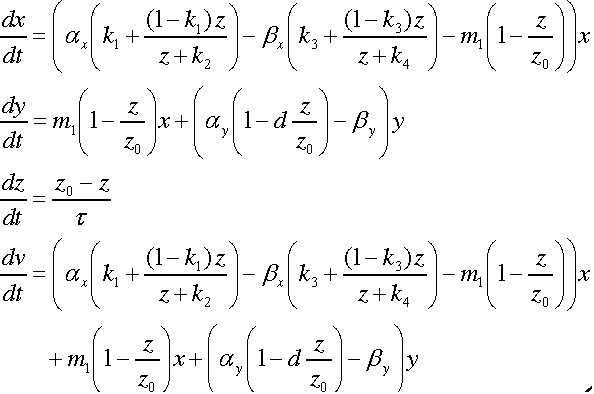
\includegraphics[width=0.45\textwidth]{images/prostatebw-mode2.pdf}
  }
  \hfill
  \subfloat[Visualization of a generated counterexample. Change in the shade of colors represents discrete mode changes.]{%
    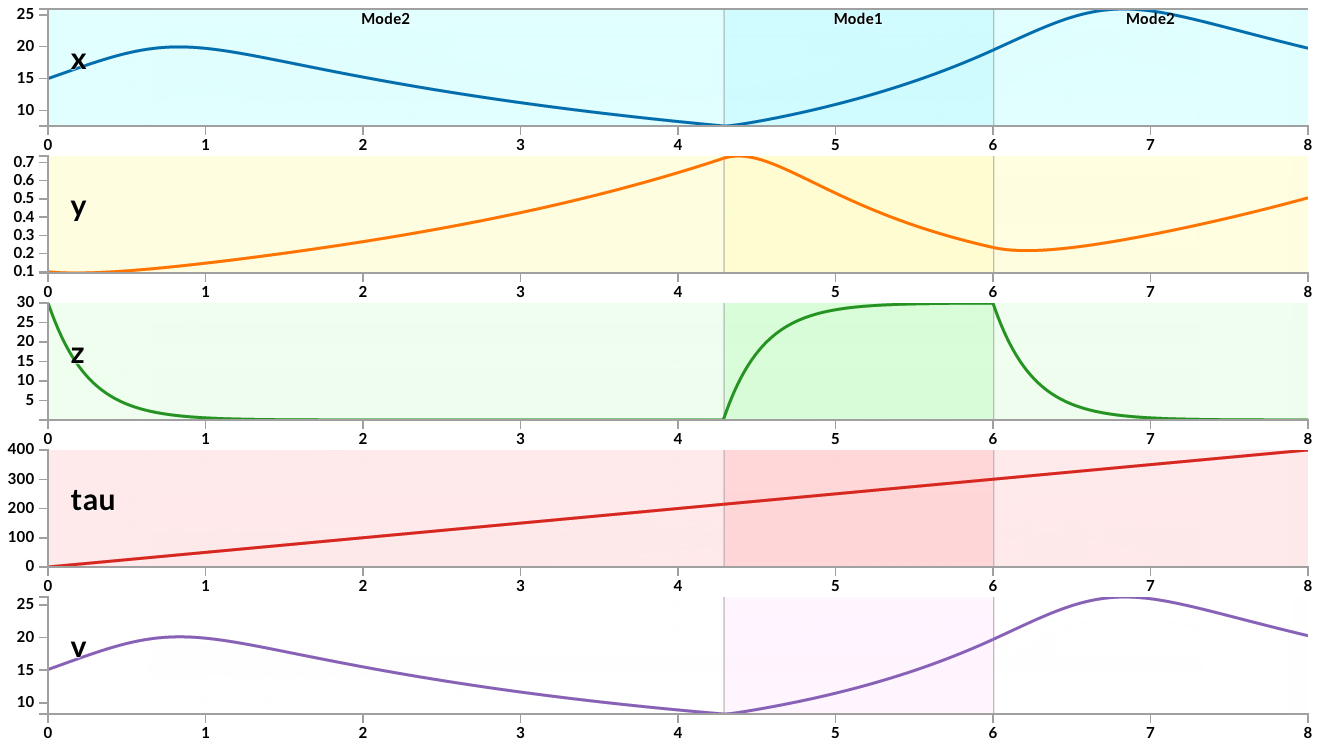
\includegraphics[width=0.48\textwidth]{images/prostate}
  }
  \caption{An example of nonlinear dynamics and counterexample-generation.}
  \label{fig:prostate-example}
\end{figure}

It is well-known that the standard bounded reachability problems for
simple hybrid systems are already highly
undecidable~\cite{DBLP:conf/hybrid/AlurCHH92}.
Instead, we work in the framework of $\delta$-reachability of hybrid systems~\cite{DBLP:journals/corr/GaoKCC14}.
Here $\delta$ is an arbitrary positive rational number, provided by the user to
specify the bound on numerical errors that can be tolerated in the analysis.
For a hybrid system $H$ and an unsafe region $\unsafe$ (both encoded as logic formulas),
the $\delta$-reachability problem asks for one of the following answers:
\begin{itemize}
        \item {\sf safe}: $H$ cannot reach $\unsafe$.
        \item {\sf $\delta$-unsafe}: $H^{\delta}$ can reach $\unsafe^{\delta}$.
\end{itemize}
Here, $H^{\delta}$ and $\unsafe^{\delta}$ encode ($\delta$-bounded) overapproximations
of $H$ and $\unsafe$, defined explicitly as their syntactic variants.%(See Section~\ref{sec:delta-reachability} in the Appendix.)
It is important to note that the definition makes the answers no weaker than standard reachability:
When {\sf safe} is the answer, we know for certain that $H$ does not reach
the unsafe region (no $\delta$ is involved); when {\sf $\delta$-unsafe} is the answer,
we know that there exists some $\delta$-bounded perturbation of the system that can render it unsafe.
Since $\delta$ can be chosen to be very small, {\sf$\delta$-unsafe} answers in fact
discover robustness problem in the system, which should be regarded as unsafe indeed.
We have proved that bounded $\delta$-reachabilty is decidable for a wide range
of nonlinear hybrid systems, even with reasonable complexity bounds~\cite{DBLP:journals/corr/GaoKCC14}.
This framework provides the formal correctness guarantees of \dReach{}.

Apart from solving $\delta$-reachability, the following key features of \dReach{}
distinguish it from other existing tools in this
domain~\cite{DBLP:journals/jlp/FranzleTE10,DBLP:conf/cav/FrehseGDCRLRGDM11,DBLP:journals/tac/AlthoffK14,DBLP:conf/hybrid/Frehse05,DBLP:conf/icons/HerdeEFT08,DBLP:conf/rtss/ChenAS12,DBLP:conf/aaai/CimattiMT12}.
%insert explanations for each item.
\begin{enumerate}
\item Expressiveness. \dReach{} allows the user to describe hybrid
  systems using first-order logic formulas over real numbers with a
  wide range of nonlinear functions. This allows the user to specify
  the continuous flows using highly nonlinear differential equations,
  and the jump and reset conditions with complex Boolean combinations
  of nonlinear constraints. \dReach{} also faithfully translates mode
  invariants into $\exists\forall$ logic formulas, which can be
  directly solved under certain restrictions on the invariants.
\item Property-guided search. \dReach{} maintains logical encodings
  (the same approach as~\cite{DBLP:conf/aaai/CimattiMT12}), whose size
  is linear in the size of the inputs, of the reachable states of a
  hybrid system~\cite{DBLP:journals/corr/GaoKCC14}. The tool searches
  for concrete counterexamples to falsify the reachability properties,
  instead of overapproximating the full reachable states. This avoids
  the usual state explosion problem in reachable set computation,
  because the full set of states does not need to be explicitly
  stored. This change is analogous to the difference between SAT-based
  model checking and BDD-based symbolic model checking.
\item Tight integration of symbolic reasoning and numerical solving.
  \dReach{} delegates the reasoning on discrete mode changes to SAT
  solvers, and uses numerical constraint solving to handle nonlinear
  dynamics. As a result, it can combine the full power of both
  symbolic reasoning and numerical analysis algorithms. In particular,
  all existing tools for reachable set computation can be easily
  plugged-in as engines for solving the continuous part of the
  dynamics, while logic reasoning tools can overcome the difficulty in
  handling complex mode transitions.
\end{enumerate}
The paper is structured as follows. We describe the system architecture in Section 2,
and give some details about the logical encoding in the tool in Section 3.
We then explain the input format and usage in Section 4. %More details and examples are given in the Appendix.

%Realistic hybrid systems involves nonlinear ODEs with transcendental
%functions. \dReach{} allows users to specify a hybrid system in a
%nonlinear signature as it is without linearizing or overapproximating
%it. Users can provide the tool with a numerical error bound $\delta$,
%a bounded time horizon $[0, T]$, and a maximum number of mode switches
%$k$ for the analysis. As a result of analysis, \dReach{} will return
%either \textbf{$\delta$-sat} with a concrete counterexample, or
%\textbf{unsat} which does not involve numerical errors. We also
%provide a visualization for the $\delta$-sat case to help
%understand the analysis result.

% TODO: Need to differentiate this paper from FMCAD paper
%  - FMCAD: underlying solving techniques for SMT with ODEs
%  - TACAS: tool, encoding, using solver...

%%% Local Variables:
%%% mode: latex
%%% TeX-master: "main"
%%% End:

% !TEX root = /Users/kquine/Dropbox/Research/Papers/2015/CPS-SMT-RTSS/cps-rtss.tex

\section{PALS Overview}
\label{sec:pals}

PALS transforms 
 a \emph{synchronous design} $\mathit{SD}$ with global period $T$
into a \emph{correct-by-construction} 
distributed real-time system $\mathcal{MA}(\mathit{SD}, T, \Gamma)$,
provided that the underlying network infrastructure give bounds %$\Gamma$ on network delays, execution times,  and clock skews, 
$\Gamma = (\epsilon, \alpha_{\min}, \alpha_{\max}, \mu_{\min}, \mu_{\max})$
with
%
\begin{inparaenum}[(i)]
	\item $\epsilon$ a maximal clock skew  with respect to the global clock,
	\item $[\alpha_{\min},\alpha_{\max}]$  bounds for processing I/O, 
	executing a transition, and real-time scheduling
	and
	\item $[\mu_{\min}, \mu_{\max}]$ bounds  for the network transmission delay.
	%between any two nodes. % in the network.
\end{inparaenum}
This section overviews the synchronous models, % $\mathit{SD}$,
the distributed  models, % $\mathcal{MA}(\mathit{SD}, T,\Gamma)$,
 and their relationship %between $\mathit{SD}$ and $\mathcal{MA}(\mathit{SD}, T,\Gamma)$
(we refer to~\cite{mr-pals-journal,pals-tcs} for details).


\subsection{Discrete Synchronous Models}

The synchronous model $\mathit{SD}$ is specified  as 
an \emph{ensemble}
$\mathcal{E}$  of %(nondeterministic)
state machines with input and output ports.
For each iteration, a machine performs a transition
based on its current state and the inputs (from other machines), %or its environment)
 proceeds to the next state, and generates new outputs for the next iteration.


\begin{definition}
A  \emph{typed machine}  $M = (D_i,S,D_o,\delta_M)$
is composed of:
%
\begin{inparaenum}[(i)]
	\item $D_i = D_{i_1} \times \cdots \times D_{i_n}$ an input set 
	(a value to the $k$-th \emph{input port}  is an element of  $D_{i_k}$), 
	% for $1 \leq k \leq n$, 
	\item $S$ a set of states, 
	\item $D_o =D_{o_1} \times \cdots \times D_{o_m}$ an output set
	(a value from the $j$-th \emph{output port} is an element of  $D_{o_j}$), and 
	% for $1 \leq j \leq m$
	\item $\delta_M \subseteq (D_i \times S) \times (S \times D_o)$ a total
	transition relation.
\end{inparaenum}  
\end{definition}




As illustrated in Fig.~\ref{fig:ensemble},
a collection $\{M_j\}_{j\in J_S\cup J_F}$ of  state machines with different periods 
can be composed into a 
\emph{multirate ensemble} $\mathcal{E}$.
The period of a slow machine $s \in J_S$ (with $\mathit{rate}(s) = 1$) is 
a multiple of the period of a fast machine $f \in J_F$ (with $\mathit{rate}(f) > 1$). 
A \emph{wiring diagram} connects  the input and output ports of the machines or the ensemble $\mathcal{E}$, %the environment,
where no connection exists between two fast machines.

\begin{figure}
\centering
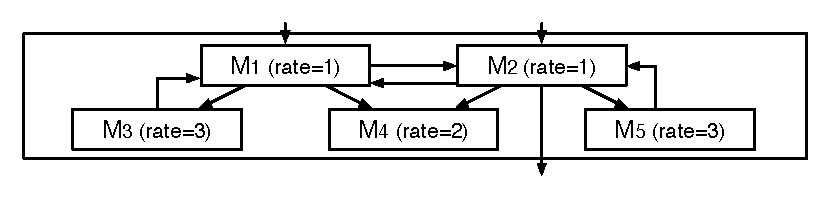
\includegraphics[clip=true,trim=0.3cm 0.4cm 0.3cm 0.4cm,width=\columnwidth]{ensemble.pdf}    
\caption{A multirate ensemble $\mathcal{E}$,
with $M_1$ and $M_2$ slow machines.
%and $M_3$, $M_4$, and $M_5$ are fast machines.
}  \label{fig:ensemble}
\end{figure}

In each iteration, all components in $\mathcal{E}$ perform the transitions \emph{in lockstep}.
A fast machine $f$ is \emph{slowed down} 
and performs $k = \mathit{rate}(f)$ internal transitions  in one global synchronous step.
Since 
a fast machine produces $k$-tuples of outputs in one step, 
%but a slow machine only needs  a single input value.
%Therefore,
\emph{input adapters} are applied 
to generate single values (e.g., the last value, or 
the average of the $k$ values) for a slow machine. 
Likewise, a single output  from a slow machine is adapted to a $k$-tuple of inputs 
for a fast machine.




The \emph{synchronous composition}  of a multirate ensemble $\mathcal{E}$
is equivalent to a single machine $M_\mathcal{E}$.
If a machine in $\mathcal{E}$ has a feedback wire connected to itself or to another component, then the output becomes an input of the destination component in the next iteration.
That is,  $M_\mathcal{E}$'s states %$S^{\mathcal{E}} = (\Pi_{j\in J} S_j) \times (\Pi_{j\in J}  D_\mathit{OF}^j)$,
consist of the states %$S_j$ 
of its subcomponents %$M_j$ 
and
the   ``feedback'' outputs. %$D_\mathit{OF}^j$ for $j \in J_S \cup J_F$
%(i.e., the outputs from  $M_j$   to some machine in $\mathcal{E}$). 
For example, 
%the synchronous composition 
$M_\mathcal{E}$ of 
%the ensemble 
$\mathcal{E}$ in Fig.~\ref{fig:ensemble} 
is the machine given by the outer box. 
%Notice that $M_\mathcal{E}$ can appear as a component 
%in another multirate ensemble, resulting in hierarchical multirate systems.


\subsection{PALS Distributed  Real-Time Models}
\label{pals-dist}

Each component in the  distributed model $\mathcal{MA}(\mathcal{E}, T, \Gamma)$
is composed of a machine in $\mathcal{E}$ and \emph{wrappers} around it, as illustrated in Fig.~\ref{fig:wrappers}.
%The outermost wrapper  is  the PALS wrapper, which encloses an input adaptor wrapper, 
%which  encloses either a (slow) machine or a $k$-machine wrapper, 
%which encloses a  (fast) machine. 
In $\mathcal{MA}(\mathcal{E}, T, \Gamma)$,
an innermost machine performs at its own rate according to its local clock
that deviates by less than $\epsilon$ from the global  clock.
At the beginning of its periods, it reads its input from the layer above, 
performs a transition, and then generates the outputs.
%when the execution of the transition is finished.

\begin{figure}
\centering
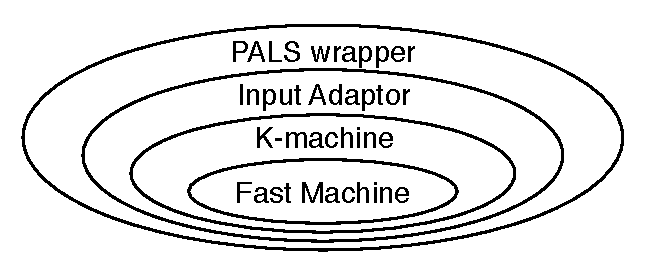
\includegraphics[width=0.49\columnwidth,clip=true,trim=0.3cm 0.3cm 0.3cm 0.3cm]{Onion-f.pdf}
\hfill
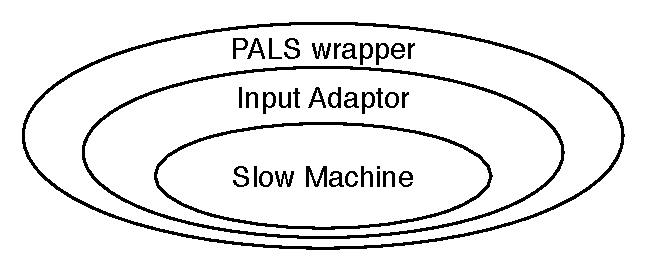
\includegraphics[width=0.49\columnwidth,clip=true,trim=0.3cm 0.3cm 0.3cm 0.3cm]{Onion-s.pdf}
\caption{The wrapper hierarchies %for fast machines (left) and slow machines (right) 
in PALS distributed real-time  models.}
\label{fig:wrappers}
\end{figure}


%
A wrapper has I/O buffers, some timers, and access to the machine's  local clock.
A PALS wrapper %communicates with the other components, and 
shares the same \emph{global period~$T$}.
Received inputs are stored in the input buffer.
When a new $i$-th round begins %according to its local clock 
(at time $u_0 \in (iT-\epsilon, iT+\epsilon)$),
it delivers the contents of its input buffer to the inner input adaptor wrapper,
and sets its \emph{backoff timer} to $2\epsilon -\mu_{min}$.
%to prevent that outputs are sent out too early.
When the execution of all the inner components is finished \emph{and}
the backoff timer expires (before $u_0 + \max(2\epsilon -\mu_{min}, \alpha_{max})$),
the contents of the output buffer are sent out, %into the network
and delivered to the destination before $u = \mu_{max} + u_0 +  \max(2\epsilon -\mu_{min}, \alpha_{max})$.
If $T\geq 2\epsilon + \mu_{max} + \max(2\epsilon -\mu_{min}, \alpha_{max})$,
then all inputs are read in a round-consistent way since $u < (i+1)T - \epsilon$.



An input adaptor wrapper reads the inputs from the PALS wrapper
and applies input adaptors %function
%to get either a single value from a $k$-tuple input  for slow machines, or
%a $k$-tuple of values from a single input for fast machines.
for each global period $T$. % according to its local clock.
A  $k$-machine wrapper
\begin{inparaenum}[(i)]
	\item extracts each value from the $k$-tuple input and delivers it to the enclosed fast machine
at each fast period $T/ k$, and
	\item delivers the $k$-\emph{tuples} from the outputs of the fast machine to its outer layer
	at each global period $T$.
\end{inparaenum}



A fast machine $M_f$ %in $\mathcal{MA}(\mathcal{E}, T, \Gamma)$ 
may \emph{not} be able to finish 
all of its $k$ internal transitions in a global  round
 \emph{before} the outputs must be sent to arrive before %the beginning of 
the next round.
The number of transitions that $M_f$ can perform before the deadline is 
 $k'= 1+\lfloor \max(T - (2\epsilon + \mu_{max} + \alpha_{max_f}), 0)\cdot (k / T)\rfloor$,
 where  $\alpha_{{\max}_f}$ is the maximal execution time for $M_f$.
If $k' < k$,
then $M_f$'s $k$-machine wrapper only sends the first $k'$ values
(followed by $k - k'$ ``don't care'' values $\bot$).
The input adaptor of each %slow machine's 
input port whose source is $M_f$
must %be \emph{$(k'+1)$-oblivious}, i.e., it 
ignores the last $k - k'$ values
$v_{k'+1}, \ldots, v_k$ in a $k$-tuple $(v_1, \ldots,  v_k)$.
%


\begin{figure}
\begin{center}
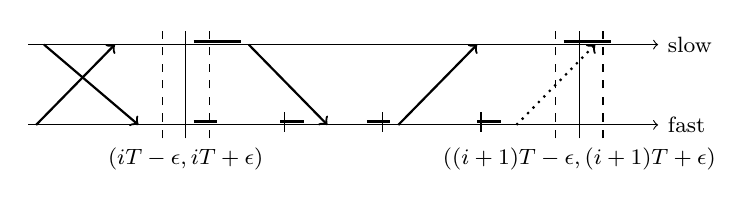
\begin{tikzpicture}[yscale=0.85,font=\footnotesize]
\draw [->] (0,0) -- (8,0) node  [right] {fast};
\draw [->] (0,1.2) -- (8,1.2) node [right] {slow};

\draw (2, -0.2) node [below] {$(i  T - \epsilon, i T + \epsilon)$} -- (2, 1.4);
\draw[dashed] (1.7, -0.2) -- (1.7, 1.4)  ;
\draw[dashed] (2.3, -0.2)  -- (2.3, 1.4);

\draw (7, -0.2) node [below] {$((i+1)  T - \epsilon, (i+1) T + \epsilon)$} -- (7, 1.4);
\draw[dashed] (6.7, -0.2)  -- (6.7, 1.4);
\draw[dashed] (7.3, -0.2)  -- (7.3, 1.4);

\draw [->,thick] (0.1, 0) -- (1.1, 1.2);
\draw [->,thick] (0.2, 1.2) -- (1.4, 0);

\draw [->,thick] (2.8, 1.2) -- (3.8, 0);
\draw [->,thick] (4.7, 0) -- (5.7, 1.2);
\draw [->,thick,dotted] (6.2, 0) -- (7.2, 1.2);

\draw [very thick] (2.1, 1.25) -- (2.7, 1.25);
\draw [very thick] (6.8, 1.25) -- (7.4, 1.25);

\draw [very thick] (2.1, 0.05) -- (2.4, 0.05); 
\draw [very thick] (3.2, 0.05) -- (3.5, 0.05); \draw (3.25, -0.1) -- (3.25, 0.2);
\draw [very thick] (4.3, 0.05) -- (4.6, 0.05); \draw (4.5, -0.1) -- (4.5, 0.2);
\draw [very thick] (5.7, 0.05) -- (6.0, 0.05); \draw (5.75, -0.1) --(5.75, 0.2);

\end{tikzpicture}
\caption{Timeline for $\mathcal{MA}(\mathcal{E}, T, \Gamma)$ ($k=4$ and $k' = 3$).
Diagonal arrows denote network transmission and short horizontal lines denote the execution.
The dotted arrow illustrates that the outputs can arrive after the beginning of the next round 
%for the slow component 
if the fast machine waits until all its transitions are finished.
\label{fig:mr-timeline}}
\end{center}
\end{figure} 



\subsection{Relating the Synchronous and Distributed Models}

In a distributed real-time model $\mathcal{MA}(\mathcal{E}, T, \Gamma)$,
network transmission can happen only in between  $(iT+\epsilon, (i+1)T-\epsilon)$
for each $i$-th period, as depicted in Fig.~\ref{fig:mr-timeline}.
Therefore, at each time $iT - \epsilon$, all the input buffers of the PALS wrappers are full, 
and all the other input and output buffers are empty.
A \emph{stable state} of the distributed model $\mathcal{MA}(\mathcal{E}, T, \Gamma)$
is a snapshot of the system at each time $iT - \epsilon$,
just before the components in $\mathcal{MA}(\mathcal{E}, T, \Gamma)$ 
start performing local machine transitions \cite{pals-tcs}.



\emph{Big-step} transitions are defined between two stable states of $\mathcal{MA}(\mathcal{E}, T, \Gamma)$,
and they are related to single steps of the synchronous composition $M_{\mathcal{E}}$.
%
There exists a function $\mathit{sync}$ 
associating each stable state with the corresponding state of $M_{\mathcal{E}}$.
%
Two stable states are related by $s_1 \sim_\mathit{obi} s_2$ iff 
their  machine states are identical
and 
their corresponding input buffer contents \emph{cannot} be
distinguished by input adaptors.  

\begin{theorem}\label{thm:mr-pals}   \cite{mr-pals-journal}
The relation $(\sim_\mathit{obi} \,;\, \mathit{sync})$ 
is a bisimulation between 
the transition system induced by $M_{\mathcal{E}}$
and the big-step stable transition system induced by $\mathcal{MA}(\mathcal{E}, T, \Gamma)$.
\end{theorem}











% !TEX root = /Users/kquine/Dropbox/Research/Papers/2015/CPS-SMT-RTSS/cps-rtss.tex

\section{Hybrid PALS}
\label{sec:hybrid-pals}


%\textbf{(Peter) Some very important overview text added!}

This section presents \emph{Hybrid PALS}, which extends PALS to hybrid
systems.  One main difference between PALS and Hybrid PALS is that
 the time at which an event takes place does not matter in PALS, as
long as it happens within a certain time interval. This
 allows us to relate a distributed
real-time system to an essentially untimed synchronous model. However,
in hybrid systems, we cannot abstract from the time at which a
continuous value is read or  an actuator command is given
(both of which depend on a node's imprecise local clocks). Therefore,
the precise times at which these events happen must be included also
in the \emph{synchronous} Hybrid PALS models to have any possibility
of a bisimulation between the synchronous model and the distributed
hybrid system. 


In Hybrid PALS, a  state of a physical environment %of a machine $M$ 
is given by 
a tuple $\vec{v} = (v_1,\ldots,v_l) \in \mathbb{R}^l$ 
of its physical parameters $\vec{x} = (x_1, \ldots,x_l)$,
and
the behavior of %the physical parameters 
$\vec{x}$
can be modeled using ODEs that specify \emph{trajectories} 
$\tau_1, \ldots, \tau_l$ of %the parameters 
$\vec{x}$ over time.
%
%The continuous dynamics %of the system 
%is specified by \emph{controlled physical environments} $E$.
The standard PALS models $\mathcal{E}$ and $\mathcal{MA}(\mathcal{E},T,\Gamma)$ 
are  nondeterministic models defined for \emph{any possible} environment behaviors.
Then,
the \emph{environment restrictions} 
$\mathcal{E} \restriction E$ and
$\mathcal{MA}(\mathcal{E},T,\Gamma)\restriction E$
%introduced in~\cite{hybrid-pals}, 
 define the behavior of the models 
 constrained by the physical  environment $E$.  To have any
 control over when values are read from, and sent to, physical environments, we add in this paper \emph{sampling and
   response timing policies} to the Hybrid PALS models. 
We then  
prove a bisimulation equivalence 
relating $\mathcal{E}\restriction E$ and $\mathcal{MA}(\mathcal{E}, T,\Gamma)\restriction E$,
%with respect to physical environments,
which generalizes the  trace equivalence result in \cite{hybrid-pals}.



\subsection{Controlled Physical Environments}

%Let $\vec{\tau}(t) = (\tau_1(t),\ldots,\tau_l(t))$
%for an l-tuple of trajectories 
%$\vec{\tau} = (\tau_1,\ldots,\tau_l)$.
%Notice that the parameters $\vec{x}$ are also trajectories
%in such a way that a state of  the physical environment at time $t$


A (local)  physical environment $E_M$ of machine $M$
is specified as a   \emph{controlled physical environment}
that defines every possible trajectory of its physical parameters $\vec{x}$
for the control commands from $M$.
%
For a state $\vec{v} \in \mathbb{R}^l$, a control command $a$, and a duration $t \in \mathbb{R}$,
a controlled physical environment $E_M$
gives a trajectory $\vec{\tau}$ of its parameters $\vec{x}$ of duration $t$,
as illustrated in Fig.~\ref{fig:physical-transition}
%(e.g., state $v_1$, command $a$, duration $t_2-t_1$ yields trajectory $\tau_1$).

\begin{definition}
Let  $\mathcal{T}$ denote the set of all
trajectories (a trajectory of duration $T$ is a function $\tau : [0,T] \rightarrow \mathbb{R}$).
A \emph{controlled physical environment} $E_M = (C, \vec{x}, \Lambda)$ consists of:
\begin{inparaenum}[(i)]
    \item $C$ a set of \emph{control commands}; %(or ``actuator outputs'') from  $M$;
    \item $\vec{x} = (x_1, \ldots,x_l)$ a vector of real number variables; and
    \item $\Lambda \subseteq (C \times \mathbb{R}_{\geq 0} \times \mathbb{R}^l) \times \mathcal{T}^l$
    a \emph{physical transition relation}, where
    $((a, t, \vec{v}),  \vec{\tau}) \in \Lambda$
    iff for a control command $a \in C$ that lasts 
    for duration~$t$, 
    $E_M$'s physical state $\vec{x}$ follows the trajectory 
    $\vec{\tau} \in \mathcal{T}^l$
    from $\vec{v} \in \mathbb{R}^l$ with
        $\vec{\tau}(0) = \vec{v}$.
\end{inparaenum}
(E.g., $((a_1,t_2-t_1,v_1), \tau_1) \in \Lambda$ in Fig.~\ref{fig:physical-transition}).
\end{definition}

\begin{figure}
\centering
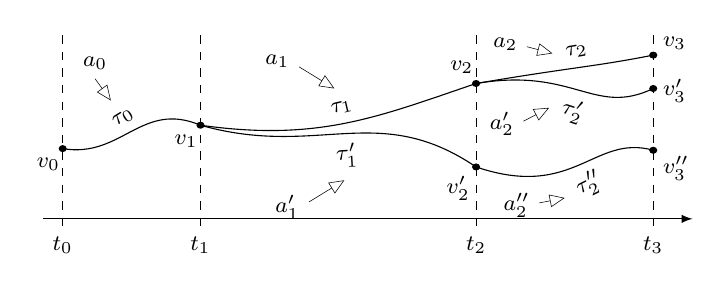
\begin{tikzpicture}[xscale=2.5,yscale=2.12,font=\footnotesize]
%baseline
\draw[-latex,thin] (-0.1,0) -- (3.2,0);
\draw[shift={(0,0)},thin,dashed] (0,1.1) -- (0,-0.05) node[below] {\footnotesize $t_0$};
\draw[shift={(0.7,0)},thin,dashed] (0,1.1) -- (0,-0.05) node[below] {\footnotesize $t_1$};
\draw[shift={(2.1,0)},thin,dashed] (0,1.1) -- (0,-0.05) node[below] {\footnotesize $t_2$};
\draw[shift={(3,0)},thin,dashed] (0,1.1) -- (0,-0.05) node[below] {\footnotesize $t_3$};
%curves
\begin{scope}[yshift=6pt]
\filldraw (0,0.21) circle (0.5pt) node[below,xshift=-1.2ex] {$v_0$};
\draw (0,0.21) .. controls (0.3,0.15) and (0.4,0.5) .. node[above,sloped] (t0) {$\tau_0$} (0.7,0.35);
\draw[-open triangle 45,very thin] ($(t0.north) + (-0.1,0.15)$) node[above] {$a_0$} -- ($(t0.north) + (-0.02,0.02)$);
    \filldraw (0.7,0.35) circle (0.5pt) node[below,xshift=-1.2ex] {$v_1$};
    \draw (0.7,0.35) .. controls (1.3,0.25) and (1.6,0.4) .. node[above,sloped] (t1) {$\tau_1$} (2.1,0.6);
    \draw[-open triangle 45,very thin] ($(t1.north) + (-0.2,0.15)$) node[left,yshift=2pt] {$a_1$} -- ($(t1.north) + (-0.02,0.02)$);
	\filldraw (2.1,0.6) circle (0.5pt) node[above,xshift=-1.2ex] {$v_2$};
	\draw (2.1,0.6) .. controls (2.6,0.7) and (2.7,0.7) .. node[above,sloped] (t2) {$\tau_2$} (3,0.77);
	\draw[-open triangle 45,very thin] ($(t2.west) + (-0.15,0.05)$) node[left,yshift=1pt] {$a_2$} -- ($(t2.west) + (-0.02,0.01)$);
	    \filldraw (3,0.77) circle (0.5pt) node[right,yshift=1ex] {$v_3$};
	\draw (2.1,0.6) .. controls (2.6,0.7) and (2.7,0.4) .. node[below,sloped] (t2') {$\tau_2'$} (3,0.57);
	    \filldraw (3,0.57) circle (0.5pt) node[right,yshift=-0.2ex] {$v_3'$};
	\draw[-open triangle 45,very thin] ($(t2'.west) + (-0.15,-0.1)$) node[left,yshift=-1pt] {$a_2'$} -- ($(t2'.west) + (-0.02,-0.02)$);

    \draw (0.7,0.35) .. controls (1.3,0.15) and (1.6,0.5) .. node[below,sloped] (t1') {$\tau_1'$} (2.1,0.1);
    \draw[-open triangle 45,very thin] ($(t1'.south) + (-0.2,-0.15)$) node[left,yshift=-2pt] {$a_1'$} -- ($(t1'.south) + (-0.02,-0.02)$);
	\filldraw (2.1,0.1) circle (0.5pt) node[below,xshift=-1.5ex] {$v_2'$};
	\draw (2.1,0.1) .. controls (2.6,-0.1) and (2.7,0.3) .. node[below,sloped] (t2''){$\tau_2''$} (3,0.2);
	\draw[-open triangle 45,very thin] ($(t2''.west) + (-0.15,-0.05)$) node[left,yshift=-1pt] {$a_2''$} -- ($(t2''.west) + (-0.02,-0.02)$);
	    \filldraw (3,0.2) circle (0.5pt) node[right,yshift=-1.5ex] {$v_3''$};;;
\end{scope}
\end{tikzpicture}
\caption{A controlled physical environment $E_M$.}
\label{fig:physical-transition}
\end{figure}


Several physical environments may be physically correlated,
and one %local 
environment may % immediately
affect  another environment.
Such %physical 
correlations are %naturally 
expressed as
\emph{time-invariant constraints} $(\forall t.\, \psi)$ of physical parameters over time $t$.
%(e.g., some parameter of one physical environment should always 
%  equal some other  parameter of another physical environment).
For example, if %physical 
parameter $x_1$ of $E_{M_1}$
must be equal to  parameter $x_2$ of %another environment 
$E_{M_2}$,
then the time-invariant constraint is  %the formula
$\forall t.\; x_1(t) = x_2(t)$.
%\footnote{Without loss of generality, we assume that different parameter names of different components are all different.}
%with variable $t$ for time.




\subsection{Environment-Restricted Controllers}
\label{sec:env-res}

A controller $M$ is a \emph{nondeterministic} machine
parameterized by any behavior of its %physical 
environment $E_M$.
%
The controller 
$M$ interacts  with %its physical environment 
$E_M$
according to its local clock,
which may  differ from global time by up to  
the maximal clock skew $\epsilon$.
Let $c_M : \mathbb{N} \to \mathbb{R}_{>0}$ denote a a \emph{periodic local clock} of $M$
that gives the \emph{global time} at the
beginning of the $(i+1)$-th period according to $M$'s local clock. 
That is,  $c_M(0) = 0$
and
$c_M(n) \in (n T - \epsilon, n T + \epsilon)$ for each $n > 0$.



\begin{figure}
\centering
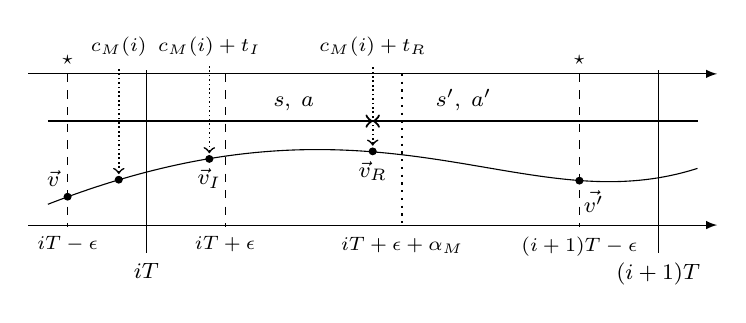
\begin{tikzpicture}[xscale=2.5,yscale=2.4,font=\footnotesize]
%baseline
\draw[-latex,thin] (-0.2,0) -- (3.3,0);
\draw[-latex,thin] (-0.2,0.8) -- (3.3,0.8);

\draw[thin] (0.4,0.82) -- (0.4,-0.15) node[below] { $iT$};
\draw[thin] (3,0.82) -- (3,-0.15) node[below] { $(i+1)T$};

\draw[->,thick] (-0.1,0.55) -- node[above,xshift=7ex] {$s,\; a$} (1.55,0.55);
\draw[<-,thick] (1.55,0.55) -- node[above,xshift=-6ex] {$s',\; a'$} (3.2,0.55);

\begin{scope}[font=\scriptsize]
\draw[dashed] (0,0.8) node[above] {$\star$} -- (0,-0.01) node[below] {$iT - \epsilon$} ;
\draw[dashed] (0.8,0.8) -- (0.8,-0.01) node[below] {$iT + \epsilon$};
\draw[dotted,thick] (1.7,0.8) -- (1.7,-0.01) node[below] {$iT + \epsilon + \alpha_M$};
\draw[dashed] (2.6,0.8) node[above] {$\star$}  -- (2.6,-0.01) node[below] { $(i+1)T - \epsilon$};

\draw[<-,densely dotted,semithick] (0.26,0.27) -- (0.26,0.84) node[above] {$c_M(i)$};
\draw[<-,densely dotted,semithick] (0.72,0.38) -- (0.72,0.84) node[above] {$c_M(i) + t_I$};
\draw[<-,densely dotted,semithick] (1.55,0.42) -- (1.55,0.84) node[above] {$c_M(i) + t_R$};
\end{scope}

\filldraw (0,0.15) circle (0.5pt) node[above,xshift=-1.2ex] {$\vec{v}$};
\filldraw (0.26,0.24) circle (0.5pt);
\filldraw (0.72,0.35) circle (0.5pt) node[below] {$\vec{v}_I$};
\filldraw (1.55,0.39) circle (0.5pt) node[below] {$\vec{v}_R$};
\filldraw (2.6,0.235) circle (0.5pt) node[below,xshift=1.2ex] {$\vec{v'}$};
\draw (-0.1,0.11) .. controls (1.6,0.8) and (2.3,0.0) .. (3.2,0.3);
\end{tikzpicture}
\caption{Timeline for an environment-restricted controller $M \restriction E_M$
with a local clock $c_M$, an environment sampling time $t_I$, and an response time $t_R$.}
\label{fig:env-restriction}
\end{figure}



Fig.~\ref{fig:env-restriction} depicts the behavior of 
the \emph{environment restriction} $M \restriction E_M$ %of  $M$ by   $E_M$ 
in a PALS distributed model. % $\mathcal{MA}(\mathcal{E},T,\Gamma)$.
Its $(i+1)$-th period begins  at time $c_M(i) \in (i T - \epsilon, i T + \epsilon)$. 
% according to its local clock $c_M$.
As explained in Section~\ref{pals-dist}, $M$ has already received all the inputs $\vec{i}$ %for this round 
before time $i T - \epsilon$.  At this time, $M$ also samples the
appropriate values of its environment $E_M$. The sampling takes time
$t_I$, so that 
the physical state $\vec{v}_I$ of $E_M$ is read at time $c_M(i) + t_I$.
$M$ executes its transition based on the inputs $\vec{i}$, the %sampled 
physical state $\vec{v}_I$,  and the current 
machine state $s$.
%
After the execution ends,
the machine state changes to  $s'$, and the new controller command $a$
is sent to $E_M$  at time  $c_M(i) + t_R$, %where it is treated immediately.
where $t_R$ denotes the response time, 
which equals the transition execution time and the actuator processing time.
The new outputs $\vec{o}$ from $M$ are delivered to their destination before $(i+1) T - \epsilon$.
%footnote{KYUNGMIN:  this last sentence is my understanding; is it correct?  We need to
%  explain clearly exactly when sampling and actuating take place, and  that's what I have tried.}




%We assume that 
A control command from a controller $M$ depends on $M$'s current 
machine state.
In Fig.~\ref{fig:env-restriction}, a current control command $a$ (given by $s$) remains effective 
until the execution ends at time $c_M(i) + t_R$,
and then a new control command $a'$ (given by $s'$) takes effect.
A physical environment 
$E_M$ defines trajectories of its parameters $\vec{x}$:
\begin{inparaenum}[(i)]
    \item from state $\vec{v}$ to $\vec{v}_I$ for the interval $[iT - \epsilon, c_M(i) + t_I]$ by the current command $a$,
    \item from $\vec{v}_I$ to $\vec{v}_R$ for the interval $[c_M(i) + t_I, c_M(i) + t_R]$ by again $a$, and 
    \item from $\vec{v}_R$ to $\vec{v'}$ for $[c_M(i) + t_R, (i+1)T-\epsilon]$ by the new control command $a'$.
\end{inparaenum}
Notice that $0 \leq t_I \leq t_R \leq \alpha_M$ for the maximal execution time $\alpha_M$  of $M$.
As a result,
a \emph{big step} transition of $M \restriction E_M$ from state $(s, \vec{v})$ with input $\vec{i}$ 
to state $(s',\vec{v'})$ with output $\vec{o}$
is defined for the time interval $[iT - \epsilon, (i+1)T-\epsilon]$ in \emph{distributed PALS models}.

% Moreover, $M \restriction E_M$ 
% can be considered as a ``normal'' state machine
% in \emph{synchronous models},
% provided that the timing values (such as $c_M(i)$, $t_I$, and $t_R$)
% as well as control commands are  determined by $M$'s machine states
% and inputs.\footnote{KYUNGMIN:  This last paragraph seems a little
%   unmotivated and misplaced here; can it be dropped?  Instead, it
%   would be MUCH better to informally introduce ``interfaces'' before
%   giving the definition ...}

A machine $M$ that integrates both a controller and its environment
should have a state space of the form $S\times \mathbb{R}^m$,  where
$\mathbb{R}^m$ is the state space of the $m$ physical parameters that
$M$ observes.   That $M$ has a transition for \emph{any} environment
values follows directly from the definitions of machines: their
transition relations are total. To compose such a machine with its
environment, we must define the ``interface'' between the controller
part and the ``environment part'' of such an environment-parametric
machine $M$. This interface is given by the following projection functions:


\begin{definition}
\label{def:env-interface}
% Suppose that $M$ has a state space of the form
% $S\times \mathbb{R}^m$  for $\mathbb{R}^m$ the $m$ physical parameters that $M$ observes.   
% For $(s,\vec{v}_o) \in S \times \mathbb{R}^m$,
The \emph{interface} of a controller $M$ is given by the %following
projection functions $\pi=(\pi_T, \pi_R, \pi_I, \pi_C, \pi_O)$, where $s\in S$ is a state in $M$: 
\begin{inparaenum}[(i)]
        \item $\pi_T(s) \in \mathbb{N}$ a ``round'' number; 
        %(i.e., $\pi_T(s) = i$ means that the next iteration of the system is iteration $i$); 
        \item $\pi_R(s,\vec{i}) \in \mathbb{R}$ a %environment 
        response time;
        \item $\pi_I(s) \in \mathbb{R}$ a %environment 
        sampling time;
        and    
        \item $\pi_C(s) \in C$ the control command of $M$  to $E_M$.
\end{inparaenum}
For state $\vec{v} \in \mathbb{R}^l$ of $E_M$,  
the \emph{observable} part of $\vec{v}$ by $M$
is given by the projection function 
$\pi_O(\vec{v}) \in \mathbb{R}^{m}$.
\end{definition}

The environment restriction of $M$ can then be defined in the expected way:
% Given state $(s, \vec{v})$ and input $\vec{i}$,
% the next state $(s', \vec{v'})$ and output $\vec{o}$ can be constructed %using $M$ and $E_M$
% by the same process of Fig.~\ref{fig:env-restriction}:

\begin{definition}
\label{def:env-res}
The \emph{environment restriction} of $M$ by $E_M$ 
with an interface $\pi$ is %the machine
$M \restriction_\pi E_M = (D_i, S \times \mathbb{R}^l, D_o, \delta_{M \restriction_\pi E_M})$,
where
$( (\vec{i}, (s,\vec{v})), ((s',\vec{v'}), \vec{o}) ) \in \delta_{M \restriction_\pi E_M}$ holds iff
 $\pi_T(s') = i + 1$ for the round number $i = \pi_T(s)$, and:
\begin{enumerate}
    \item %(Sampling) 
    $((a,u_I,\vec{v}),\tau_I) \in \Lambda$ and $\vec{v}_I = \tau_I(u_I)$,
    for  $t_I = \pi_I(s)$, duration $u_I = (c_M(i)+t_I)-(iT-\epsilon)$, and
    the current controller command $a = \pi_C(s)$;

    \item %(Execution) 
    $((a,u_R-u_I,\vec{v}_I),\tau_R) \in \Lambda$ and $\vec{v}_R = \tau_R(u_R-u_I)$,
    for $t_R = \pi_R(s,\vec{i})$ and $u_R = (c_M(i)+t_R) - (iT-\epsilon)$;

    \item %(Transition) 
    $( (\vec{i}, (s,\pi_O(\vec{v}_I))), ((s',\pi_O(\vec{v'})), \vec{o}) ) \in \delta_{M}$; and
    
    \item %(Waiting) 
    $((a',T - u_R,\vec{v}_R),\tau_W) \in \Lambda$ and  $\vec{v'} = \tau_W(T - u_R)$,
    for the next control command $a' = \pi_C(s')$.
\end{enumerate}
\end{definition}



\subsection{Hybrid PALS}

Hybrid PALS models are parameterized by \emph{sampling and response timing policies}
that 
determine sensor sampling timing $t_I$ and actuator response timing $t_R$.
%besides  bounds $\Gamma$.
Such a policy 
is given as a collection of 
projection functions $\pi=(\pi_T, \pi_R, \pi_I, \pi_C, \pi_O)$ 
in Definition~\ref{def:env-interface}.
The continuous dynamics %of a PALS system 
is ``completely'' decided  
by the controllers % (in $\mathcal{E}$ or $\mathcal{MA}(\mathcal{E},T,\Gamma)$),
their physical environments, and timing policies (including local clocks of controllers). 
%  \textbf{(Peter)  Are the clock functions also parameters, or are we quantifying over
%  all local clock skews??}


Deciding $\pi$ is a design choice. 
% Most generally, values of $\pi$ can vary
% according to states and inputs.
% More realistically, sampling/response timings are fixed 
% to certain numbers to simplify the system complicity.
In % our previous work
\cite{hybrid-pals}, $t_I$ is $0$ 
(for controllers tightly integrated with its environments)
and $t_R$ is  
the maximum execution time $\alpha_{\max}$.


The synchronous model in Hybrid PALS is specified
as a multirate ensemble $\mathcal{E}$ and  the physical environments of subcomponents,
where physical correlations between those environments
are specified as time-invariant constraints.

\begin{definition}
A \emph{hybrid multirate ensemble} $\mathcal{E}\restriction_{\Pi} E_{\mathcal{E}}$
is given by:
\begin{inparaenum}[(i)]
    \item a multirate ensemble $\mathcal{E}$, %= (J_S ,  J_F, e, \{M_j\}_{j\in J_S \cup J_F}, E, \mathit{src}, \mathit{rate}, \mathit{adap})$ 
    \item a family of policy functions $\Pi=\{\pi_j\}_{j\in J_S  \cup J_F}$
    (with $J_S$ an index set of slow machines and $J_F$ an index set of fast machines),
    and
    \item a family of local physical environments 
    $E_\mathcal{E} = \langle\{E_{M_j}\}_{j\in J_S \cup J_F}, \forall t.\, \psi)\rangle$ 
    with $\forall t.\,\psi$ the time-invariant constraints.
\end{inparaenum}
\end{definition}   


The behaviors of a hybrid ensemble  $\mathcal{E} \restriction_{\Pi} E_\mathcal{E}$
are  a \emph{subset} of the behaviors of $\mathcal{E}$, namely, the behaviors restricted by 
the physical environment $E_\mathcal{E}$.
As mentioned,
each (decelerated) environment-restricted machine $M_j \restriction_\pi E_{M_j}$ defines 
a transition from a state  at time $iT - \epsilon$ to one at time $(i+1)T-\epsilon$ for a global period $T$.
Therefore, a lock-step composition of such %environment-restricted 
transitions
\emph{that also satisfy the time-invariant constraints} gives a transition of 
the synchronous composition $M_{\mathcal{E} \restriction_{\Pi} E_\mathcal{E}}$
from one state at time $iT - \epsilon$ to another state at time $(i+1)T-\epsilon$.


Hybrid PALS maps a hybrid multirate ensemble
$\mathcal{E}\restriction_{\Pi} E_\mathcal{E}$ with a global period $T$, 
together with PALS bounds $\Gamma$,  to the distributed hybrid system  
$\mathcal{MA}(\mathcal{E}, T, \Gamma) \restriction_{\Pi} E_\mathcal{E}$.
Similarly, its  behaviors are the subset of those of the %PALS
distributed system $\mathcal{MA}(\mathcal{E}, T, \Gamma)$ that can be realized
by the %physical 
environment $E_\mathcal{E}$
and satisfy the time-invariant constraints.
In particular, big-step transitions of each component $M_j \restriction_\pi E_{M_j}$ are
defined for the interval $[iT - \epsilon, (i+1)T-\epsilon]$
 as explained in Section~\ref{sec:env-res}.


The correctness of Hybrid PALS follows from the fact that 
all physical measurements and physical activation \emph{happen at the same time}
in both $\mathcal{E} \restriction_{\Pi} E_\mathcal{E}$  and $\mathcal{MA}(\mathcal{E}, T, \Gamma) \restriction_{\Pi} E_\mathcal{E}$ with the \emph{same timing policies} $\Pi$.
%(see Definition~\ref{def:env-res}).
%
Recall that stable states of $\mathcal{MA}(\mathcal{E}, T, \Gamma)$ are states at times $iT - \epsilon$.
Hence,  big-step ``stable'' transitions are well defined for 
$\mathcal{MA}(\mathcal{E}, T, \Gamma) \restriction_{\Pi} E_\mathcal{E}$
from $iT - \epsilon$ to $(i+1)T-\epsilon$,
which are exactly related to single steps of the synchronous composition 
$M_{\mathcal{E} \restriction_{\Pi} E_\mathcal{E}}$ (by the same relation $(\sim_\mathit{obi} \,;\, \mathit{sync})$ in Theorem~\ref{thm:mr-pals}).
Consequently, we have:


\begin{theorem}\label{thm:hybrid-pals} 
The relation $(\sim_\mathit{obi} \,;\, \mathit{sync})$ 
is a bisimulation between 
the transition system by $\mathcal{E} \restriction_{\Pi} E_\mathcal{E}$ 
and the big-step stable transition system induced by $\mathcal{MA}(\mathcal{E}, T, \Gamma) \restriction_{\Pi} E_\mathcal{E}$.
\end{theorem}






% !TEX root = /Users/kquine/Dropbox/Research/Papers/2015/CPS-SMT-RTSS/cps-rtss.tex


\section{Logical Encoding of Hybrid PALS Models}
\label{sec:smt-encoding}

Thanks to the behavioral equivalence (Theorem~\ref{thm:hybrid-pals}),
analysis problems of a distributed CPS $\MA(\mathcal{E}, T, \Gamma) \restriction_{\Pi} E_\mathcal{E}$
are reduced to those on the simpler synchronous model $\mathcal{E} \restriction_{\Pi} E_\mathcal{E}$.
%Directly analyzing such distributed systems is unfeasible in practice
%due to the combinatorial explosion even for simple discrete systems \cite{pals-tcs}.
However, it is difficult to analyze $\mathcal{E} \restriction_{\Pi} E_\mathcal{E}$ 
with (nonlinear)  continuous dynamics and skews of the local clocks.
% (bounded by $\epsilon > 0$).
The concrete values of local clocks are unknown since the values %of local clocks 
are determined on-the-fly by  \emph{clock synchronization} mechanisms \cite{pals-rtss09,lynch-book}.
Numerical simulation can no longer be used for nonlinear dynamics
because numerical errors can be accumulated.

This section explains how analysis problems of 
$\mathcal{E}\restriction_{\Pi}E_\mathcal{E}$ for \emph{any possible local clock}
can be symbolically encoded as logic formulas over the real numbers and ODEs.
The satisfiability of such formulas can then be automatically decided by SMT solving up to a given precision $\delta > 0$
(see Section~\ref{sec:smt-logic}).
%The idea is to express synchronous transitions in $\mathcal{E} \restriction_{\Pi} E_\mathcal{E}$ 
%as formulas of the form $\phi(\vec{i}, \vec{y} \shortmid \vec{y'}, \vec{o})$, where 
%\begin{inparaenum}[(i)]
%	\item $\vec{i}$ denotes the inputs, 
%	\item $\vec{y}$ denotes the states  at the beginning of the round at time $iT - \epsilon$,
%	\item $\vec{y'}$ denotes the states at the end of the round at time $(i+1)T - \epsilon$, and 
%	\item $\vec{o}$ denotes the outputs.
%\end{inparaenum}
%Using $\phi(\vec{i}, \vec{x} \shortmid \vec{x'}, \vec{o})$ as building blocks,
%we show formulas for bounded analysis, inductive analysis, 
%and compositional analysis of parameterized systems.


\subsection{Representing Environment-Restricted Controllers}
\label{sec:discrete-encoding}

A controller $M$ is naturally 
expressed as a logic formula over discrete domain
of the form $\phi_M(\vec{i}, \vec{y} \shortmid \vec{y'}, \vec{o})$,
including \emph{variables}
$\vec{i}$ denoting input, 
$\vec{y}$ denoting the current state, 
$\vec{y'}$ denoting the next state, and 
$\vec{o}$  denoting output.

\begin{definition}
For  $M = (D_i,S,D_o,\delta_M)$,
the formula $\phi_M$ is defined as
$\phi_{M}(\vec{d}_i, s \shortmid s',  \vec{d}_o)
\iff
( (\vec{d}_i, s), (s', \vec{d}_o) ) \in \delta_{M}$.
\end{definition}



A physical environment $E_M$ is expressed as 
a formula over the real numbers %and ODEs
of the form $\phi_{E_M}(\vec{a},u_0,u_t,\vec{v} \shortmid \vec{x})$,
including: \begin{inparaenum}[(i)]
	\item \emph{unary function symbols} $\vec{x}$ denoting the trajectories of $E_M$'s physical parameters $\vec{x}$,
	and
	\item \emph{variables} $\vec{a}$ denoting control commands, % from its controller $M$, 
		$u_0$ and $u_t$ respectively denoting 
		times at the beginning and the end of the trajectory duration, and 
		$\vec{v}$ denoting initial values of the trajectories $\vec{x}$ at time $u_0$.
\end{inparaenum}


If the continuous dynamics of $\vec{x}$ is specified as a system of ODEs
$\frac{\mathrm{d}\vec{x}}{\mathrm{d}t}= F_{\vec{a}}(\vec{x},t)$
for a control command $\vec{a}$, then the formula $\phi_{E_M}$ 
includes universal quantification over time along with solutions of the ODEs, such as a formula of the form:
\[
\bigvee \big(\mathit{guard}(\vec{a}) \rightarrow
\forall t \in [u_0,u_t].\;
\vec{x}(t) = \vec{v} + \int_0^{t-u_0} \!  F_{\vec{a}}(\vec{x},t)\,\mathrm{d}t
\big)
\]
For example, 
the formula $\phi_{E_M}(\mathit{rate}_M,u_0,u_t,v_M \shortmid \alpha_M)$
for 
%an environment 
$E_M$ of a subcontroller $M$ in the airplane example is given by:
$\forall t \in [u_0, u_t].\; \alpha_M(t) = v_M + \int_0^{t-u_0}  \mathit{rate}_M \,\mathrm{d}t$.
%where the surface angle $\alpha_M$ follows the ODE
%$\frac{\mathrm{d}\alpha_M}{\mathrm{d}t} = \mathit{rate}_M$
%from the current angle $v_M$ in the time interval $[0,u]$.


\begin{definition}
For %a physical environment 
$E_M = (C, \vec{x}, \Lambda)$,
%the formula $\phi_{E_M}$ is defined as
$\phi_{E_M}(\vec{a},u_0,u_t,\vec{v} \shortmid \vec{x})$
iff
$((\vec{a},u_t-u_0,\vec{v}), \vec{\tau}) \in \Lambda$
and $\vec{x}(t) = \vec{\tau}(t - u_0)$ for $t \in [u_0, u_t]$.
\end{definition}


For an environment restriction $M \restriction E_M$,
its formula $\phi_{M \restriction E_M}$ 
has the form
$\phi_{M \restriction E_M}^{T,i}(\vec{i}, \vec{y}, \vec{v} \shortmid \vec{y'}, \vec{v'}, \vec{o})$,
including variables:
\begin{inparaenum}[(i)]
	\item $\vec{i}$ denoting input, 
	\item $(\vec{y},\vec{v})$ denoting a state  at the beginning of the round 
		(at time $iT - \epsilon$),
	\item $(\vec{y'},\vec{v'})$ denoting a state at the end of the round 
		(at time $(i+1)T - \epsilon$), and 
	\item $\vec{o}$ denoting output.
\end{inparaenum}
%
Instead of explicitly writing $iT - \epsilon$ and $(i+1)T - \epsilon$  in $\phi_{M \restriction E_M}$,
we use the ``$\epsilon$-shifted''  time axis for the interval $[iT, (i+1)T]$. %for the formula $\phi_{M \restriction E_M}$.
%
%A formula $\phi_{M \restriction E_M}$ 
%is basically the direct translation of its formal definition in Definition~\ref{def:env-res}.
But due to clock skews, 
the exact values of sampling time $u_I = (c_M(i)+t_I)-(iT-\epsilon)$
and response time $u_R = (c_M(i)+t_R)-(iT-\epsilon)$ are unpredictable. 
Because $iT - \epsilon < c_M(i) < iT + \epsilon$,
we represent those times as formulas 
$t_I < u_I < t_I + 2\epsilon$ and $t_R < u_R < t_R + 2\epsilon$
within $\phi_{M \restriction E_M}$.






\begin{definition}
For an environment restriction $M \restriction E_M$
with the interface projection functions $\pi=(\pi_T, \pi_R, \pi_I, \pi_C, \pi_O)$,
%the formula 
$\phi_{M \restriction E_M}^{T,i}(\vec{i}, \vec{y}, \vec{v} \shortmid \vec{y'}, \vec{v'}, \vec{o})$
is defined from Definition~\ref{def:env-res} by:
\begin{align*}
\begin{alignedat}{3}
\exists \vec{a},\vec{a'}, \vec{v}_I, \vec{v}_R, u_I, u_R, t_I, t_R.\;
&&&
\vec{a} = \pi_C(\vec{y})
\\
\wedge\;
\phi_{E_M}(\vec{a},iT,iT+u_I,\vec{v} \shortmid \vec{x})
&\;\;\wedge\;\;&&
\vec{v}_I = \vec{x}(iT+u_I)
\\
\wedge\;
\phi_{E_M}(\vec{a},iT+u_I,iT+u_R,\vec{v}_I \shortmid \vec{x})
&\;\;\wedge\;\;&&
\vec{v}_R = \vec{x}(iT+u_R)
\\
\wedge\;
\phi_M(\vec{i},\langle\vec{y},\pi_O(\vec{v}_I)\rangle \shortmid \langle\vec{y'},\pi_O(\vec{v'})\rangle, \vec{o})
&\;\;\wedge\;\;&&
\vec{a'} = \pi_C(\vec{y'})
\\
\wedge\;
\phi_{E_M}(\vec{a'},iT+u_R, (i+1)T ,\vec{v}_R \shortmid \vec{x})
&\;\;\wedge\;\;&&
\vec{v'} = \vec{x}((i+1)T)
\\
\wedge\;
t_I = \pi_I(\vec{y})
&\;\;\wedge\;\;&&
t_R = \pi_R(\vec{y},\vec{i})
\end{alignedat}
\\
\begin{alignedat}{3}
\wedge\;
(t_I < u_I < t_I + 2\epsilon)
\;\wedge\;
(t_R < u_R < t_R + 2\epsilon)
\end{alignedat}
\end{align*}
%
Notice that a local clock $c_M$ (and the round number $\pi_T$)
are abstracted from the formula.
That is,
$\phi_{M \restriction E_M}(\vec{i}, s, \vec{v} \shortmid s', \vec{v'}, \vec{o})$
iff
$( (\vec{i}, (s,\vec{v})), ((s',\vec{v'}), \vec{o}) ) \in \delta_{M \restriction E_M}$
for some $c_M$.
\end{definition}




\subsection{Representing Hybrid Ensembles}

%Recall that 
A synchronous composition  of %an ensemble 
$\mathcal{E}$ is a single machine $M_\mathcal{E}$
in which all machines perform their transitions in lock step.
Each fast machine $f$  performs $k = \mathit{rate}(f)$  internal transitions in one step.
%
A formula 
$\phi_{(M \restriction E_M)^{\times k}}^{T, i}$
for the $k$-step \emph{deceleration} of an environment restriction 
$M \restriction E_M$
is defined by sequentially 
composing
$k$ subformulas $\phi_{M \restriction E_M}^{T/k,ik},\ldots,\phi_{M \restriction E_M}^{T/k,(ik+k-1)}$.
These formulas are respectively related to the $k$ equal \emph{subintervals} $[(ik+n-1)T/k-\epsilon,(ik+n)T/k-\epsilon]$ 
for $n=1,\ldots,k$.

\begin{definition}
Given $M \restriction E_M$ and $k \in \mathbb{N}$,
the formula
$\phi_{(M \restriction E_M)^{\times k}}^{T, i}(\langle\vec{i_1},\ldots,\vec{i_k}\rangle, \vec{y_0}, \vec{v_0} \shortmid \vec{y}_{k}, \vec{v}_{k}, \langle\vec{o_1},\ldots,\vec{o_k}\rangle)$ is:
\[
%(\exists \vec{y_1},\ldots, \vec{y}_{k-1}, \vec{v_1},\ldots, \vec{v}_{k-1})
\exists\{\vec{y_n}, \vec{v_n}\}_{n=1}^{k-1}.\,
\bigwedge_{n=1}^k \phi_{M \restriction E_M}^{T/k,(ik+n-1)}(\vec{i_n}, \vec{y}_{n-1}, \vec{v}_{n-1} \shortmid \vec{y_{n}}, \vec{v_{n}}, \vec{o}_n)
\]
\end{definition}

The wiring diagram of $\mathcal{E}$ is expressed by
a conjunction of %appropriate 
\emph{equalities} between variables denoting input and output ports.
Each equality corresponds to a connection in $\mathcal{E}$
(together with an input adaptor for machines with different rates).
%Since feedback outputs of one machine to itself or another machine 
%becomes input of their destinations in the next step,
%we use a separate set of variables for such output ports connected to other machines in $\mathcal{E}$.
%$\phi_\mathit{wire}$ is a conjunction of equalities, together with the input adaptors of $\{M_j\}_{j\in J_S\cup J_F}$,  given by the wiring diagram of $\mathcal{E}$.


\begin{definition}
%The formula 
$\phi_\mathit{wire}$ is the conjunction of the equalities:
\begin{inparaenum}[(i)]
	\item $\alpha_j^l(i_j^l) = i_e^n$
	for each connection from $\mathcal{E}$'s $n$-th input port to $M_j$'s $l$-th input port 
	with its input adaptor $\alpha_j^l$;
	\item $o_e^n = o_j^l$
	for each connection from $M_j$'s $l$-th output port to $\mathcal{E}$'s $n$-th output port; and
	\item $\alpha_j^l(i_j^l) = f_k^n$ and ${f_k^n}' = o_k^n$
	for each connection from $M_k$'s $n$-th output port to $M_j$'s $l$-th input port with its input adaptor $\alpha_j^l$,
	where $f_k^l$ denotes a feedback output from the previous step, 
	and ${f_k^l}'$ denotes one for the next step.
\end{inparaenum}
\end{definition}


For a hybrid ensemble $\mathcal{E} \restriction_{\Pi} E_\mathcal{E}$ 
of machines  $\{M_j\}_{j\in J_S\cup J_F}$ and their physical environments $\{E_{M_j}\}_{j\in J_S\cup J_F}$
($J_S$ denoting slow machines and $J_F$ denoting fast machines),
its formula has the form
$\phi_{\mathcal{E} \restriction_{\Pi} E_\mathcal{E}}^{T,i}(
	\vec{i}, \{\vec{z_j},\vec{f_j}\}_{j\in J_S\cup J_F}
	\shortmid 
	\{\vec{z'_j}, \vec{f_j'}\}_{j\in J_S\cup J_F}, \vec{o})$,
%
including variables:
\begin{inparaenum}[(i)]
	\item $\vec{i}$ denoting input, 
	\item $\vec{z_j}$ denoting a state of $M_j \restriction E_{M_j}$ at the beginning of the round 
		(at time $iT - \epsilon$),
	\item $\vec{f_j}$ denoting feedback outputs from the previous round,
	\item $\vec{z_j'}$ denoting a state of $M_j \restriction E_{M_j}$ at the end of the round 
		(at time $(i+1)T - \epsilon$), 
	\item $\vec{f_j'}$ denoting the feedback outputs for the next round,	and 
	\item $\vec{o}$ denoting output.
\end{inparaenum}


\begin{definition}
For a hybrid ensemble $\mathcal{E} \restriction_{\Pi} E_\mathcal{E}$, %of machines 
%$\{M_j\}_{j\in J_S\cup J_F}$, their physical environments $\{E_{M_j}\}_{j\in J_S \cup J_F}$
%and the time-invariant constraint $(\forall t.\; \psi)$,
its formula
$\phi_{\mathcal{E} \restriction_{\Pi} E_\mathcal{E}}^{T,i}(
	\vec{i}, \{\vec{y_j}, \vec{v_j},\vec{\mathit{f}_j}\}_{j\in J_S\cup J_F}
	\shortmid 
	\{\vec{y'_j}, \vec{v'_j}, \vec{\mathit{f}_j'}\}_{j\in J_S\cup J_F}, \vec{o})$ is:
\begin{align*}
%(\exists \{\vec{i_j},\vec{o_j}\}_{j\in J_S\cup J_F})\;
\exists \{\vec{i_j},\vec{o_j}\}_{j\in J_S\cup J_F}.\;
\textstyle\bigwedge_{s \in J_S}
\big(\phi_{M_s \restriction E_{M_s}}^{T,i}(\vec{i_s}, \vec{y_s}, \vec{v_s} \shortmid \vec{y'_s}, \vec{v'_s}, \vec{o}_s)\big)
\phantom{.}
\\
\wedge\;
\textstyle\bigwedge_{f \in J_F}
\big(\phi_{(M_f \restriction E_{M_f})^{\times\mathit{rate}(j)}}^{T,i}(\vec{i_f}, \vec{y_f}, \vec{v_f} \shortmid \vec{y'_f}, \vec{v'_f}, \vec{o}_f)\big)
\phantom{.}
\\
\wedge\;
\phi_\mathit{wire}(\vec{i},\vec{o},\{\vec{i_j},\vec{o_j},\vec{\mathit{f}_j},\vec{\mathit{f}_j'}\}_{j\in J_S\cup J_F})
\;\wedge\;
(\forall t.\; \psi).
\end{align*}
\end{definition}

By construction, a formula $\phi_{\mathcal{E} \restriction_{\Pi} E_\mathcal{E}}^{T,i}$ is satisfiable
iff there is a corresponding transition of the synchronous composition $M_{\mathcal{E} \restriction_{\Pi} E_\mathcal{E}}$
from $iT - \epsilon$ to $(i+1)T - \epsilon$ for \emph{some} local clocks.
Therefore, by  the bisimulation equivalence (Theorem~\ref{thm:hybrid-pals}):

\begin{theorem}\label{thm:pals-encoding}
$\phi_{\mathcal{E} \restriction_{\Pi} E_\mathcal{E}}^{T,i}$ is satisfiable 
iff for some local clocks, there exists a corresponding \emph{stable transition} in a distributed hybrid system  
$\MA(\mathcal{E}, T, \Gamma) \restriction_{\Pi} E_\mathcal{E}$   for $[iT - \epsilon,(i+1)T - \epsilon]$.
\end{theorem}

\subsection{Representing Formal Analysis Problems}

Our goal is to verify safety properties
of a distributed CPS $\MA(\mathcal{E}, T, \Gamma) \restriction_{\Pi} E_\mathcal{E}$.
In general, a safety property of the system can be expressed as a formula of the form 
$\forall t.  \mathit{safe}(\vec{z},t)$
with respect to state variables $\vec{z}$ and time variable $t$.


For bounded analysis
to verify %whether $\MA(\mathcal{E}, T, \Gamma) \restriction_{\Pi} E_\mathcal{E}$
a safety property %$\forall t.  \mathit{safe}(\vec{z},t)$
up to a given bound $n \in \mathbb{N}$
(i.e., for the interval $[0,nT - \epsilon]$),
we encode its \emph{bounded counterexamples}. %of $\forall t.  \mathit{safe}(\vec{z},t)$
%up to the bound $n$.
If the formula is unsatisfiable (i.e., no counterexample), 
then the system satisfies the safety property in $[0,nT - \epsilon]$
\emph{for any local clocks} by Theorem~\ref{thm:pals-encoding}.



\begin{definition}
A bounded analysis problem for $\forall t.  \mathit{safe}(\vec{z},t)$
%of $\MA(\mathcal{E}, T, \Gamma) \restriction_{\Pi} E_\mathcal{E}$ 
up to $n$ with an initial condition $\mathit{init}(\vec{z})$
is expressed by:
\begin{align*}
\exists \vec{z}_0, \{\vec{z}_k, \vec{i}_k, \vec{o}_k, t_k\}_{k=1}^{n}.\;
\textstyle\bigwedge_{k=1}^{n}
\big(\phi_{\mathcal{E} \restriction_{\Pi} E_\mathcal{E}}^{T,k}(
	\vec{i}_k, \vec{z}_{k-1}
	\shortmid 
	\vec{z}_{k}, \vec{o}_k)\big)
\phantom{.}
\\
\wedge\;
\mathit{init}(\vec{z}_0)
\;\wedge\;
\textstyle\bigvee_{k=1}^{n}
\big(
(k-1)T < t_{k} \leq T
\wedge
\neg\mathit{safe}(\vec{z}_k, t_{k}) 
\big).
\end{align*}
\end{definition}


For unbounded verification of a safety property,
we encode its inductive proof as logic formulas.
The idea is to find an inductive condition $\mathit{ind}(\vec{z})$ 
for synchronous transitions
that corresponds to the beginning of a global round,
and to show that $\mathit{ind}(\vec{z})$ implies %the safety property 
$\mathit{safe}(\vec{z},t)$ 
for that round.

\begin{definition} 
An inductive analysis problem for $\forall t.  \mathit{safe}(\vec{z},t)$
with an inductive condition $\mathit{ind}(\vec{z})$ is expressed by:
\begin{multline*}
\forall \vec{z}, \vec{z'}, \vec{i}, \vec{o}, t \in [0,T].\;
\big(\mathit{ind}(\vec{z})  \rightarrow \mathit{safe}(\vec{z},t)\big)
\\
\wedge\;
\big(
(\mathit{ind}(\vec{z})\;\wedge\;\phi_{\mathcal{E} \restriction_{\Pi} E_\mathcal{E}}^{T,0}(\vec{i}, \vec{z}\shortmid \vec{z'}, \vec{o}))
\rightarrow
\mathit{ind}(\vec{z'})\big)
.
\end{multline*}
\end{definition}

We also encode a divide-and-conquer proof
to verify a safety property by compositional analysis. % as formulas.
An input condition $\mathit{c}_\mathit{in}(\vec{i},\vec{z},t)$
and an output condition $\mathit{c}_\mathit{out}(\vec{o},\vec{z},t)$ 
during a global round
are identified for synchronous transitions
in such a way 
that $\mathit{c}_\mathit{in}(\vec{i},\vec{z},t)$ implies %the safety property 
$\mathit{safe}(\vec{z},t)$ for that round.
%(time variable $t$ is included because of time-invariant constraints).
%This method is very useful for parameterized systems (see Section~\ref{sec:case-studies}).


\begin{definition} A compositional analysis for $\forall t.  \mathit{safe}(\vec{z},t)$
with I/O conditions $\mathit{c}_\mathit{in}(\vec{i},\vec{z},t)$ and $\mathit{c}_\mathit{out}(\vec{o},\vec{z},t)$
is expressed by:
\begin{multline*}
\forall \vec{z}, \vec{z'}, \vec{i}, \vec{o}, t \in [0,T].\;
\big(\mathit{c}_\mathit{in}(\vec{i},\vec{z},t) \rightarrow \mathit{safe}(\vec{z},t) \big)
\phantom{.}
\\
\wedge\;
\big(
(\mathit{c}_\mathit{in}(\vec{i},\vec{z},t)
\;\wedge\;
\phi_{\mathcal{E} \restriction_{\Pi} E_\mathcal{E}}^{T,0}(
	\vec{i}, \vec{z}
	\shortmid 
	\vec{z'}, \vec{o})
)
\rightarrow
\mathit{c}_\mathit{out}(\vec{o},\vec{z'},t)\big).
\end{multline*}
\end{definition}

The validity of such formulas for inductive or compositional  analysis can also be automatically checked 
using SMT solving
by checking the unsatisfiability of their \emph{negations}.










% !TEX root = /Users/kquine/Dropbox/Research/Papers/2015/CPS-SMT-RTSS/cps-rtss.tex


\section{SMT Solving for Distributed CPS}
\label{sec:smt-logic}

Various formal analysis problems of distributed CPSs 
can be encoded as logic formulas over the real numbers and ODEs.
%and we are interested in using SMT solving 
%to automatically check the satisfiability of those formulas.
%
The satisfiability of those formulas is undecidable for nonlinear hybrid systems  in general,
but becomes \emph{decidable} %up to any given precision $\delta > 0$ 
if we take account of robustness properties %of the system 
under numerical perturbations $\delta > 0$.
%
A \emph{$\delta$-complete decision procedure} for a formula $\phi$ returns false 
if $\phi$ is unsatisfiable, and returns true if its syntactic 
numerical perturbation of $\phi$ by bound $\delta$ is satisfiable. 
This is practically very useful since 
sampling exact values of physical parameters is not possible in reality. 

However, formulas for hybrid PALS models
may contain ODEs and universal quantification over \emph{uninterpreted real functions},
%such as  \emph{time-invariant constraints} $(\forall t.\; \psi)$.
%in order to precisely specify physical interactions between distributed components
%with clock skews and delays.
which are not supported by current state-of-the-art SMT solving techniques.
%
For example, the ODEs in $E_\mathit{Main}$ %for the main controller 
in the airplane example
include uninterpreted function symbols $\delta_L$, $\delta_V$, and $\delta_R$ for control angles.
The correspondences between  %the angles 
$(\delta_L, \delta_V, \delta_R)$ 
and the surface angles $(\alpha_L,\alpha_V,\alpha_R)$ of the subcontrollers
are given by the time-invariant constraint
$\forall t.\, (\delta_L(t) = \alpha_L(t)) \wedge (\delta_V(t) = \alpha_V(t)) \wedge (\delta_R(t) = \alpha_R(t))$.


This section shows how formulas for hybrid PALS models (presented in Section~\ref{sec:smt-encoding})
can be equivalently encoded as \emph{SMT formulas}
without the use of universal quantification over uninterpreted real functions.
For this purpose, we present a new  SMT framework to provide 
an efficient SMT algorithm
for  formulas generated from hybrid PALS models.

%\textbf{difficulties for dealing with unint. func. sym.?}
%
%A conflict-based 
%
%It is not easy to \emph{statically check without} $\delta$-complete decision procedures
%whether such subformulas of the form $\forall t \in [0,T].\; g(t) = \mathit{flow}_q(\vec{x})(t)$
%are $\delta$-consistent to each other or not.
%
%Even though two real functions
%$f_1(t)$ and $f_2(t)$ have completely different forms, 
%their corresponding formulas 
%can be consistent up to a given precision $\delta > 0$.
%E.g.,
%for $f_1(t) = \sqrt{t+1}$ and $f_2(t) = 1 + \frac{1}{2}t - \frac{1}{8}t^2 + \frac{1}{16}x^3$,
%where $f_2(t)$ is the third order taylor expansion of $\sqrt{t+1}$,
%the formulas 
%$\forall t \in [0,T].\; g(t) = f_1(t)$ and  $\forall t \in [0,T].\; g(t) = f_2(t)$
%are consistent up to precision $\delta = 0.1$ for $T = 0.8$,
%but not consistent if  $\delta = 0.01$.
%
%We need the underlying $\mathcal{T}$-solver
%to decide their consistency up to $\delta > 0$
%(e.g., by checking the unsatisfiability of the formula
%$\exists t \in [0,T].\; f_1(t) \neq f_2(t)$).


\subsection{Theory of the Real Numbers with Function Names}

SMT-based techniques for hybrid systems
normally use the standard SMT theory of the real numbers and computable %(nonlinear) 
real functions,
such as polynomials, exponentiation, trigonometric functions,  
and solutions of Lipschitz-continuous ODEs.

\begin{definition}
For a finite set $\mathcal{F}$ of computable real functions,
%(real number constants are given as $0$-ary functions).
%
$\mathcal{L}_\mathcal{F} = (\mathcal{F}, >)$ denotes the first-order signature over the real numbers
with the functions in $\mathcal{F}$,
and $\mathbb{R}_\mathcal{F} = (\mathbb{R}, \mathcal{F}^\mathbb{R}, >^\mathbb{R})$
is the standard structure of the theory of the real numbers.
\end{definition}


Solutions of ODEs are considered as \emph{atomic functions} in $\mathcal{L}_\mathcal{F}$,
and therefore the structure of ODEs cannot be used for SMT algorithms  in this logic.
This restrictive syntax makes it difficult to efficiently express logic formulas for hybrid PALS models 
in $\mathcal{L}_\mathcal{F}$. 
% which typically involve different local physical environments interacting with each other.
%Therefore, 
We present a new SMT theory,
by extending $\mathcal{L}_\mathcal{F}$, that allows to express solutions of ODEs in a modular way,
so that the size of the formula can be much reduced.


We consider a \emph{two-sorted} first-order logic with sorts $\mathit{Real}$ and $\mathit{Name}$,
where $\mathit{Real}$ denotes the real numbers,
and $\mathit{Name}$ denotes \emph{name constants} 
for unary functions composed of the functions in $\mathcal{F}$.
For example, given $\{1, +, \times, \sin, x, y\} \subset \mathcal{F}$
and two name constants $\mathtt{m_1}$ and $\mathtt{m_2}$ of sort $\mathit{Name}$,
we can have two \emph{named} real functions:
$[\mathtt{m_1}]:
(\sin(x(t)) :\mathit{Real} \to \mathit{Real})$
and
$[\mathtt{m_2}]:
([y(t) + 1, z(t)^2] :  \mathit{Real} \to \mathit{Real}^2)$.


The new logic 
includes
a collection of \emph{application operators} $\mathit{app}^n : \mathit{Name} \times \mathit{Real} \to \mathit{Real}^n$
that connect a name constant to its underlying function with range $\mathit{Real}^n$, e.g.,
\[
\mathit{app}^1(\mathtt{m_1}, 3) \equiv \sin(x(3)),
\quad
\mathit{app}^2(\mathtt{m_2}, u) \equiv [y(u) + 1,z(u)^2].
\]
%These operators ensure that each name object is really related to a concrete unary real function with domain $\mathbb{R}$.
 

In the new logic,  we take into account
a collection of \emph{integral operators} 
$\mathit{int}^{k_1,\ldots,k_n} :  \mathit{Real} \times \mathit{Name}^n  \to \mathit{Real}^{\sum_{i=1}^n k_i}$.
An integral term
$\mathit{int}^{k_1,\ldots,k_n}(u,\nu_1,\ldots,\nu_n)$
takes time value $u$
and a list of name constants $\nu_1,\ldots,\nu_n$,
to respectively denote real functions $f_1,\ldots,f_n$ with ranges $\mathit{Real}^{k_1},\ldots,\mathit{Real}^{k_n}$,
and returns the value $\int_0^u \, [f_1(t),\ldots,f_n(t)] \,\mathrm{d}t$.  
For example:
\begin{align*}
\mathit{int}^{2}(1, \mathtt{m_2}) 
&\equiv
\int_0^1
[y + 1, z^2]
\mathrm{d}t,
\\
\mathit{int}^{1,2}(T,\mathtt{m_1},\mathtt{m_2}) 
&\equiv
\int_0^T
[\sin(x),y + 1,z^2]
\mathrm{d}t.
\end{align*}









\begin{definition}
For a  set $\mathcal{N}$ of name constants
and a set  $\mathcal{O}$ of operators  $\mathit{app}^n$ and  $\mathit{int}^{k_1,\ldots,k_n}$,
the first order signature is given by 
$\mathcal{L}_{\mathcal{F}\cup\mathcal{N}} = (\mathcal{F} \cup \mathcal{N} \cup \mathcal{O}, >)$.
%
The first order structure is given by
$\mathbb{R}_{\mathcal{F}\cup\mathcal{N}} 
= (\mathbb{R} \cup N, \mathcal{F}^\mathbb{R} \cup \mathcal{N}^N \cup \mathcal{O}^{N,\mathbb{R}}, >^\mathbb{R})$
for a fixed finite set $N$ of \emph{name objects},
where the interpretation $\mathcal{N}^N$ of name constants and 
the interpretation $\mathcal{O}^{N,\mathbb{R}}$ of application and integral operators 
are given as explained above.
%
The syntax and semantics of $\mathcal{L}_{\mathcal{F}\cup\mathcal{N}}$-formulas 
is defined by means of $\mathcal{L}_{\mathcal{F}\cup\mathcal{N}}$ and $\mathbb{R}_{\mathcal{F}\cup\mathcal{N}}$
in the standard way.
%(The signature $\mathcal{L}_\mathcal{F}$ is a subsignature of $\mathcal{L}_{\mathcal{F}\cup\mathcal{N}}$,
%and the structure $\mathbb{R}_\mathcal{F}$ for the real numbers 
%is a substructure of $\mathbb{R}_{\mathcal{F}\cup\mathcal{N}}$).
\end{definition}




The satisfiability problems of $\mathcal{L}_{\mathcal{F}\cup\mathcal{N}}$-formulas in the new theory 
$\mathbb{R}_{\mathcal{F}\cup\mathcal{N}}$
can be reduced to ones in the standard theory $\mathbb{R}_\mathcal{F}$ at minimal cost,
provided that all $\mathit{Name}$ variables %in the formulas 
are only existentially quantified.
Consider an $\mathcal{L}_{\mathcal{F}\cup\mathcal{N}}$ formula 
$\exists \vec{n}.\; \psi(\vec{n})$, where 
$\vec{n}$ are only variables of sort $\mathit{Name}$ %in $\psi(\vec{n})$
and
$\psi(\vec{n})$ contains no quantifier for $\vec{n}$.
Since there are only a finite number of name objects in $\mathbb{R}_{\mathcal{F}\cup\mathcal{N}}$,
by using the standard SMT solving for equalities,
we can enumerate all \emph{consistent} assignments 
$\vec{n} = \overrightarrow{\mathit{name}}_1,\ldots,\vec{n} = \overrightarrow{\mathit{name}}_N$ for $\vec{n}$.
Let $\hat{\psi}_i$ be the formula obtained from $\psi(\vec{n})$
by replacing each name by its related function according to the $i$-th assignment $\vec{n} = \overrightarrow{\mathit{name}}_i$.
Then, $\vee_{i=1}^N \hat{\psi}_i$ is an ordinary $\mathcal{L}_\mathcal{F}$ formula
whose satisfiability can be decided by %existing SMT techniques, such as 
$\delta$-complete decision procedures. Therefore:


\begin{theorem}\label{thm:new-dec}
The satisfiability of $\mathcal{L}_{\mathcal{F}\cup\mathcal{N}}$ formulas of the form $\exists \vec{n}.\; \psi(\vec{n})$
is decidable by  $\delta$-complete SMT solving. 
\end{theorem}


%\begin{figure}
%\begin{algorithmic}
%\STATE $V\gets$ AllUnigramsInTraining($D$)
%\STATE $N\gets$ NumberOfTweets($D$)
% \FORALL{$c \in C$}
%  \STATE $N_c \gets$ Number of tweets in Class $c$
%  \STATE ...
%  \STATE $Tweets_c \gets $All Tweets in class $c$
%  \FORALL{$t \in V$}
%    \STATE $T_ct$ = No. of times term $t$ appeared in $Tweets_c$
%  \ENDFOR
%  \FORALL{$t \in V$}
%    \STATE ...
%  \ENDFOR
%\ENDFOR
%\end{algorithmic}
%\end{figure}


%We first find a truth assignment for the names, and 
%replace names in ODEs by them
%We have a truth assignment that includes only $\mathcal{L}_\mathcal{F}$-terms.
%The satisfiability of such $\mathcal{L}_\mathcal{F}$-assignments
%can then be decided by using $\delta$-decision procedures as usual.





\subsection{SMT Encoding of Hybrid PALS Models}


We now show how hybrid PALS models
are encoded in the new SMT logic $\mathcal{L}_{\mathcal{F}\cup\mathcal{N}}$
without the use of uninterpreted real functions and universal quantification.
The idea is to construct a \emph{global} ODE formula $\phi_{\mathit{ODE}}$
that defines the combined systems of ODEs for all physical environments
in $\mathcal{E} \restriction_{\Pi} E_\mathcal{E}$.
The formula $\phi_{\mathit{ODE}}$ is parameterized by the behaviors of 
the subcomponents by means of integral operators and \emph{name variables}.
The behavior of each subcomponent $M_j \restriction E_{M_j}$ is then
specified in a modular way by assigning to each name variable an appropriate name constant for $M_j \restriction E_{M_j}$.

%First, 
We restrict our attention to time-invariant constraints \emph{with only equality terms},
such as one for the airplane example,
since physical correlations for CPS can be expressed using equality conditions in practice.
Equality  constraints, such as $x_1(t) = x_2(t)$,  can be removed
from the formula  by replacing one side with another, e.g., by replacing $x_1$ with  $x_2$.
From now on we assume that time-invariant constraints are already removed from the formula 
by this process.



Suppose that %the formula 
$\phi_{\mathcal{E} \restriction_{\Pi} E_\mathcal{E}}^{T,i}$ 
%for $\mathcal{E} \restriction_{\Pi} E_\mathcal{E}$
includes $N$ terms of the form $\vec{x_j}(u)$ to obtain a value of some parameter of $E_{M_j}$.
%We only need to use ODEs for finding those values %of all such terms
%to determine the satisfiability of $\phi_{\mathcal{E} \restriction_{\Pi} E_\mathcal{E}}^{T,i}$.
A global ODE formula $\phi_{\mathit{ODE}}$
is defined as a conjunction of $N$ ODEs for these access times
that include all sampling and response times for each (decelerated) subcomponent in a global round.
% of $\mathcal{E} \restriction_{\Pi} E_\mathcal{E}$.

\begin{definition}
Let
\begin{inparaenum}[(i)]
	\item $\vec{t} = \{t_0,t_1,\ldots,t_N\}$ be  $N$ \emph{time variables} 
	with $iT = t_0 \leq t_1 \leq t_2 \leq \cdots \leq t_N = (i+1)T$;
%
	\item $\vec{f} = \{f_j^1,\ldots,f_j^N\}_{j \in J_S \cup J_F}$ be \emph{name variables} 
	denoting $E_{M_j}$'s continuous behaviors during each interval $[t_{i-1},t_i]$;
%
	\item $\vec{g} = \{\vec{g}_0,\ldots,\vec{g}_N\}$ be \emph{global value variables}
	denoting the values of all physical parameters of $\mathcal{E} \restriction_{\Pi} E_\mathcal{E}$ at each time $t_i$; and
%
	\item $\vec{l} = \{l_j\}_{j \in J_S \cup J_F}$ denote the \emph{dimension}
	of each $E_{M_j}$'s parameters $\vec{x_j} = (x_j^1,\ldots,x_j^{l_j})$.
\end{inparaenum}
The formula
$\phi_{\mathit{ODE}}(\vec{f},\vec{t},\vec{g})$ is: %$\mathcal{L}_{\mathcal{F}\cup\mathcal{N}}$-
$\bigwedge_{1 \leq i \leq N}\;
(\vec{g}_{i} = \vec{g}_{i-1} + 
\mathit{int}^{\vec{l}}(t_{i} - t_{i-1}, \{f_j^i\}_{j \in J_S \cup J_F}))$.
\end{definition}


\begin{figure}
\centering
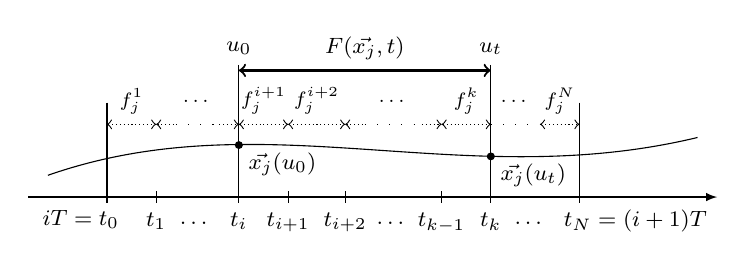
\begin{tikzpicture}[xscale=2.5,yscale=2.4,font=\footnotesize]
%baseline
\draw[-latex,thin] (-0.2,0) -- (3.3,0);

\draw[thin] (0.2,0.5) -- (0.2,-0.03) node[below,xshift=-2.2ex,yshift=0.15ex] { $iT = t_0$};
\draw[thin] (0.45,0.03) -- (0.45,-0.03) node[below] { $t_1$};
\path (0.65,-0.08) node[below] {\ldots};
\draw[thin] (1.12,0.03) -- (1.12,-0.03) node[below] { $t_{i+1}$};
\draw[thin] (1.41,0.03) -- (1.41,-0.03) node[below] { $t_{i+2}$};
\path (1.65,-0.08) node[below] {\ldots};
\draw[thin] (1.9,0.03) -- (1.9,-0.03) node[below] { $t_{k-1}$};
\path (2.35,-0.08) node[below] {\ldots};
\draw[thin] (2.6,0.5) -- (2.6,-0.03) node[below,xshift=4.7ex,,yshift=0.23ex] { $t_N = (i+1)T$};

\draw[thin] (0.87,0.7) node[above] {$u_0$}-- (0.87,-0.03) node[below] { $t_i$};
\draw[thin] (2.15,0.7) node[above] {$u_t$} -- (2.15,-0.03) node[below] { $t_{k}$};

\draw[<->,thick] (0.87,0.67) -- node[above] {$F(\vec{x_j},t)$} (2.15,0.67);

\begin{scope}[font=\scriptsize,yshift=-0.1ex]
\draw[<->,densely dotted] (0.2,0.40) -- node[above] {$f_j^1$} (0.45,0.40) ;
\draw[<-,densely dotted] (0.45,0.40) -- (0.55,0.40);
\draw[loosely dotted] (0.55,0.40) -- node[above,yshift=1ex] {\ldots} (0.77,0.40) ;
\draw[->,densely dotted] (0.77,0.40) -- (0.87,0.40);
\draw[<->,densely dotted] (0.87,0.40) -- node[above] {$f_j^{i+1}$} (1.12,0.40) ;
\draw[<->,densely dotted] (1.12,0.40) -- node[above] {$f_j^{i+2}$} (1.41,0.40) ;
\draw[<-,densely dotted] (1.41,0.40) -- (1.51,0.40);
\draw[loosely dotted] (1.51,0.40) -- node[above,yshift=1ex] {\ldots} (1.8,0.40) ;
\draw[->,densely dotted] (1.8,0.40) -- (1.9,0.40);
\draw[<->,densely dotted] (1.9,0.40) -- node[above] {$f_j^{k}$} (2.15,0.40) ;
\draw[loosely dotted] (2.15,0.40) -- node[above,yshift=1ex] {\ldots} (2.4,0.40) ;
\draw[<->,densely dotted] (2.4,0.40) -- node[above] {$f_j^{N}$} (2.6,0.40) ;
\end{scope}
\begin{scope}[yshift=0.1ex]
%\filldraw (0.2,0.19) circle (0.5pt) node[below,xshift=0.8ex] {$\vec{v}$};
\filldraw (0.87,0.26) circle (0.5pt) node[right,yshift=-1.6ex] {$\vec{x_j}(u_0)$};
\filldraw (2.15,0.2) circle (0.5pt) node[right,yshift=-1.6ex] {$\vec{x_j}(u_t)$};
%\filldraw (2.6,0.21) circle (0.5pt) node[below,xshift=1.1ex] {$\vec{v'}$};
\draw (-0.1,0.1) .. controls (1,0.5) and (2,0) .. (3.2,0.3);
\end{scope}
\end{tikzpicture}
\caption{$\mathcal{L}_{\mathcal{F}\cup\mathcal{N}}$-transformation for ODEs}
\label{fig:flow-map}
\end{figure}


For any subcomponent $M_j \restriction E_{M_j}$,
an ODE subformula $\forall t \in [u_0,u_t].\; \vec{x_j}(t) = \vec{v_j} + \int_0^{t-u_0} \!  F(\vec{x_j},t)\,\mathrm{d}t$ 
%in $\phi_{\mathcal{E} \restriction_{\Pi} E_\mathcal{E}}^{T,i}$
is replaced by conditions for variables  $\vec{f}$, $\vec{t}$, and $\vec{g}$.
For example, if $u_0 = t_i$ and $u_t = t_k$ for some $0 \leq i \leq k \leq n$,
then all $f_j^l$ for $i \leq l < k$ 
%between $t_i$ and $t_k$
denote
%are equal to the name constant $\mathtt{m}_{F(\vec{x_j},t)}$ for 
the function $F(\vec{x_j},t)$,
as illustrated in Fig.~\ref{fig:flow-map}.


\begin{definition}\label{def:ode-trans}
Let  $\pi_j(\vec{g}_i)$ denote $E_{M_j}$'s parameter values 
in the global values $\vec{g}_i$. % of $\mathcal{E} \restriction_{\Pi} E_\mathcal{E}$.
Consider an ODE formula %for $M_j \restriction E_{M_j}$ 
of the form 
$\forall t \in [u_0,u_t].\, \vec{x_j}(t) = \vec{v_j} + \int_0^{t-u_0} \!  F(\vec{x_j},t)\,\mathrm{d}t$.
If a name constant $\mathtt{m}_{F(\vec{x_j},t)}$ denotes $F(\vec{x_j},t)$,
its $\mathcal{L}_{\mathcal{F}\cup\mathcal{N}}$-formula is: % defined by the $\mathcal{L}_{\mathcal{F}\cup\mathcal{N}}$-formula:
\[
\bigvee_{0 \leq i \leq k \leq n} 
\left[
\begin{aligned}
(t_i = u_0) \wedge (t_k = u_t) \wedge \textstyle\bigwedge_{l=i}^{k-1} f^l_j \equiv \mathtt{m}_{F(\vec{x_j},t)}  ) &\;\wedge
\\
(\vec{x_j}(u_0) = \pi_j(\vec{g}_i) = \vec{v_j}) \wedge  (\vec{x_j}(u_t) = \pi_j(\vec{g}_k))
\end{aligned}
\right]
\]
\end{definition}

Let $\mathit{tr}(\phi_{\mathcal{E} \restriction_{\Pi} E_\mathcal{E}}^{T,i})$ 
be the formula
obtained from $\phi_{\mathcal{E} \restriction_{\Pi} E_\mathcal{E}}^{T,i}$ 
by repeatedly performing the $\mathcal{L}_{\mathcal{F}\cup\mathcal{N}}$-transformation
for each ODE subformula.
Finally, we obtaine the $\mathcal{L}_{\mathcal{F}\cup\mathcal{N}}$-formula 
$\tilde{\phi}_{\mathcal{E} \restriction_{\Pi} E_\mathcal{E}}^{T,i}
\equiv
\exists (\vec{f}, \vec{t}, \vec{g}).\; \phi_{\mathit{ODE}}(\vec{f},\vec{t},\vec{g}) \wedge \mathit{tr}(\phi_{\mathcal{E} \restriction_{\Pi} E_\mathcal{E}}^{T,i})$
that includes no uninterpreted real functions and universal quantification.
Therefore, the  satisfiability of $\tilde{\phi}_{\mathcal{E} \restriction_{\Pi} E_\mathcal{E}}^{T,i}$ can be determined by using
$\delta$-complete SMT (by Theorem~\ref{thm:new-dec}).


\begin{theorem}
$\phi_{\mathcal{E} \restriction_{\Pi} E_\mathcal{E}}^{T,i}$
is satisfiable
iff
%the $\mathcal{L}_{\mathcal{F}\cup\mathcal{N}}$-formula 
$\tilde{\phi}_{\mathcal{E} \restriction_{\Pi} E_\mathcal{E}}^{T,i}$
is satisfiable.
\end{theorem}

\begin{proof}[Proof Sketch]
\begin{inparaenum}
	\item[$(\Rightarrow)$]
	If $\phi_{\mathcal{E} \restriction_{\Pi} E_\mathcal{E}}^{T,i}$ is satisfiable,
	then there exists a collection $\{\vec{x_j}\}_{j \in J_S \cup J_F}$ of trajectories 
	for a global round, and we can find the values of $(\vec{f}, \vec{t}, \vec{g})$
	from the trajectories.
	\item[$(\Leftarrow)$]
	If $\tilde{\phi}_{\mathcal{E} \restriction_{\Pi} E_\mathcal{E}}^{T,i}$ is satisfiable,
	then there exist resulting values of $(\vec{f}, \vec{t}, \vec{g})$.
	Then,
	by construction, 
	any ODE subformula
	$\forall t \in [u_0,u_t].\, \vec{x_j}(t) = \vec{v_j} + \int_0^{t-u_0} \!  F(\vec{x_j},t)\,\mathrm{d}t$ is true
	iff its transformed formula by Definition~\ref{def:ode-trans} is true,
	provided that $u_0 = t_i$ and $u_t = t_k$ for some $0 \leq i \leq k \leq n$.
\end{inparaenum}
\end{proof}









% !TEX root = /Users/kquine/Dropbox/Research/Papers/2015/CPS-SMT-RTSS/cps-rtss.tex

%
\section{Case Studies and Experimental Results}
\label{sec:case-studies}

This section gives an overview of some 
case studies using Hybrid PALS and SMT-based analysis to verify %and experimental results 
distributed CPSs. 
%
These case studies involve nontrivial (nonlinear) ODEs,
due to the  continuous physical interaction between distributed components.
We have verified safety properties 
using %bounded reachability, 
inductive and compositional SMT encodings
for \emph{any possible} set of  local clocks  maximal clock skew $\epsilon$.
%
All  experiments in this section
were conducted on an Intel Xeon 2.0 GHz with 64 GB memory.
%running 64-bit Ubuntu 12.04.5 LTS.
%We set a timeout of 30 hours. % for the experiments.
The case studies and the experimental evaluation are available at %the
%\textsf{dReal} tool webpage
\url{http://dreal.github.io/benchmarks/networks}. 




\subsection{Turning an Airplane}
\label{sec:ex-airplane}

We consider a multirate distributed CPS
to turn an airplane (adapted from \cite{ftscs-journal}).
%in which a \emph{main controller} directs \emph{subcontrollers} for the ailerons and the rudder in a synchronous way.
%
To make a turn, an aircraft rolls towards the direction of the turn
by moving its \emph{ailerons} % (surfaces attached to the end of the wings).
The rolling causes 
a yawing moment in the opposite direction, called \emph{adverse yaw},
which is countered by using its \emph{rudder} (a surface attached to the vertical stabilizer).
%
The subcontrollers for the ailerons and the rudder operate at different rates, 
and the main controller orchestrates them to achieve a smooth turn.
%
Fig.~\ref{fig:airplane-ctrl} illustrates the multirate ensemble $\mathcal{E}$ of our system.


\begin{figure}
\centering
\tikzstyle{comp}=[draw,thick,rounded corners=4pt,text centered]
\tikzstyle{env}=[draw,dashed,rounded corners=8pt,text centered]
\tikzstyle{conn}=[thick,-latex,font=\scriptsize]
\tikzstyle{envconn}=[very thin,-open triangle 45,font=\scriptsize]
\begin{tikzpicture}[scale=0.9,every node/.style={transform shape},font=\footnotesize]
%components
\node (main) [comp,text width=8ex,minimum height=13ex] {{Main} ($60\, \mathrm{ms}$, $\mathit{rate}$ = $1$)}; 
\path (main.east) + (16ex,8ex) node (left) [comp,text width=14ex] {{Left aileron} ($15\,\mathrm{ms}$, $\mathit{rate}$ = $4$)}; 
\path (main.east) + (16ex,1.3ex) node (vert) [comp,text width=14ex] {{Rudder}\\ ($20\, \mathrm{ms}$, $\mathit{rate}$ = $3$)}; 
\path (main.east |- main.-48) + (16ex,0ex) node (right) [comp,text width=14ex] {{Right aileron} ($15\,\mathrm{ms}$, $\mathit{rate}$ = $4$)}; 
%comp connections
\draw [conn,latex-] (main.west |- main.north) + (3ex,0)-- node{ }+(3ex,2ex) node[above] {$\mathit{goal}_\psi$};
\draw [conn] (main.east |- main.north) + (-3ex,0)-- node{ }+(-3ex,2ex) node[above] {$\psi$};
\draw[conn] ($(main.48)+(0,0.5ex)$) -- node[above,sloped] {$\mathit{goal}_L$} ($(left.west |- left)+(0,0.5ex)$);
\draw[conn] ($(left.west |- left)+(0,-0.5ex)$) -- node[below,sloped] {$v_L$} ($(main.48)+(0,-0.5ex)$);
\draw[conn] ($(main.east)+(0,0.5ex)$) -- node[above,sloped] {$\mathit{goal}_V$} ($(vert.west |- vert)+(0,0.5ex)$);
\draw[conn] ($(vert.west |- vert)+(0,-0.5ex)$) -- node[below,sloped] {$v_V$} ($(main.east)+(0,-0.5ex)$);
\draw[conn] ($(main.-48)+(0,0.5ex)$) -- node[above,sloped] {$\mathit{goal}_R$} ($(right.west |- right)+(0,0.5ex)$);
\draw[conn] ($(right.west |- right)+(0,-0.5ex)$) -- node[below,sloped] {$v_R$} ($(main.-48)+(0,-0.5ex)$);
%physical envs
\path (main.west) + (-8ex,0ex) node (main-env) [env,text width=6ex,minimum height=13ex] {$E_\mathit{Main}$}; 
\path (left.east) + (12ex,0ex) node (left-env) [env,text width=7ex,minimum height=5ex] {$E_\mathit{Left}$}; 
\path (vert.east) + (12ex,0ex) node (vert-env) [env,text width=7ex,minimum height=5ex] {$E_\mathit{Rudder}$}; 
\path (right.east) + (12ex,0ex) node (right-env) [env,text width=7ex,minimum height=5ex] {$E_\mathit{Right}$}; 
%physical env conns
\draw[envconn] ($(main-env.east)+(0,4.5ex)$) -- node[above] {$\psi$} ($(main.west |- main-env)+(0,4.5ex)$);
\draw[envconn] (main-env.east) -- node[above] {$\phi$} (main.west);
\draw[envconn] ($(main-env.east)+(0,-4.5ex)$) -- node[above] {$\beta$} ($(main.west |- main-env)+(0,-4.5ex)$);
\draw[envconn] ($(left.east |- left-env)+(0,0.5ex)$) -- node[above] {$\mathit{rate}_L$} ($(left-env.west |- left-env)+(0,0.5ex)$);
\draw[envconn] ($(left-env.west |- left-env)+(0,-0.5ex)$) -- node[below] {$\alpha_L$} ($(left.east |- left-env)+(0,-0.5ex)$);
\draw[envconn] ($(vert.east |- vert-env)+(0,0.5ex)$) -- node[above] {$\mathit{rate}_\mathit{V}$} ($(vert-env.west |- vert-env)+(0,0.5ex)$);
\draw[envconn] ($(vert-env.west |- vert-env)+(0,-0.5ex)$) -- node[below] {$\alpha_V$} ($(vert.east |- vert-env)+(0,-0.5ex)$);
\draw[envconn] ($(right.east |- right-env)+(0,0.5ex)$) -- node[above] {$\mathit{rate}_\mathit{R}$} ($(right-env.west |- right-env)+(0,0.5ex)$);
\draw[envconn] ($(right-env.west |- right-env)+(0,-0.5ex)$) -- node[below] {$\alpha_R$} ($(right.east |- right-env)+(0,-0.5ex)$);
\end{tikzpicture}
\caption{The distributed controllers for turning an airplane.} \label{fig:airplane-ctrl}
\end{figure}


Each subcontroller $M$ gradually moves its surface towards the goal
angle $\mathit{goal}_M$ specified by the main controller
$M_\mathit{Main}$. 
In each round, $M$ receives $\mathit{goal}_M$ from $M_\mathit{Main}$,
determines the moving rate $\mathit{rate}_M$ based on $\mathit{goal}_M$ 
and the current sampled value $v_M$ of the surface angle $\alpha_M$,
and sends back $v_M$ to $M_\mathit{Main}$
(e.g., the new value of $\mathit{rate}_M$ can be given by
$ \sign(\mathit{goal}_M - v_M) \cdot \min(\abs(\mathit{goal}_M - v_M) / T, \mathit{max}_M)$).
The continuous dynamics of $\alpha_M$ is specified 
by the local physical environment $E_M$
as the ODE $\frac{\mathrm{d}\alpha_M}{\mathrm{d}t} = \mathit{rate}_M$.
%\footnote{$E_M$ is the controlled physical environment $E_M = (\mathbb{R}, \alpha_M, \Lambda_M)$
%with $((\mathit{rate}_M,T,v_M),\tau) \in \Lambda_M$ iff 
%$\tau(t) = v_M + \int_0^t  \mathit{rate}_M \,\mathrm{d}t$ for $t \in [0, T]$.}

The main controller $M_\mathit{Main}$ determines the goal angles for the subcontrollers to make a coordinated turn.
In  each round, $M_\mathit{Main}$ receives a  desired direction $\mathit{goal}_\psi$ %of the airplane 
(from the pilot)
and the surface angles $(v_L, v_V, v_R)$ from the subcontrollers, 
and then sends back the new goal angles $(\mathit{goal}_L,\mathit{goal}_V,\mathit{goal}_R)$,
%to the subcontrollers,
based on the current sampled \emph{position} values $(v_\psi, v_\phi, v_\beta)$ 
of  the direction angle $\psi$, the roll angle $\phi$, and the yaw angle $\beta$.


We consider a simple control logic to decide 
the new goal angles $(\mathit{goal}_L,\mathit{goal}_V,\mathit{goal}_R)$,
by three control functions \cite{ftscs-journal}:
%
\begin{inparaenum}[(i)]
	\item $f_\phi(v_\phi, v_\psi, \mathit{goal}_\psi)$
		returns the goal roll angle $\mathit{goal}_\phi$,
		%based on the sampled roll angle $v_\phi$, the sampled direction $v_\psi$, 
		%and the goal direction $\mathit{goal}_\psi$;
	\item $f_{R}(v_\phi, \mathit{goal}_\phi)$ returns the goal angle $\mathit{goal}_R$ for the right aileron
	(where the goal angle $\mathit{goal}_L$ for the left aileron is the opposite angle $- \mathit{goal}_R$);
	%the left aileron angle is %always  exactly opposite to the right aileron angle); 
	and
	\item $f_V(v_\beta)$ returns the goal rudder angle $\mathit{goal}_V$.
	%based on the sampled yaw angle $v_\beta$. % (the goal yaw angle is $0^\circ$).
\end{inparaenum}
For example, for $h = 0.32  (\mathit{g}_\psi - v_\psi)$:
\begin{align*}
f_\phi(v_\phi, v_\psi, g_\psi) &= 
v_\phi + \sign(h - v_\phi) \cdot \min(\abs(h - v_\phi),1.5)
\\
f_{R}(v_\phi, g_\phi) &=
\sign(\mathit{g}_\phi - v_\phi)\cdot \min(0.3 \,\abs(\mathit{g}_\phi - v_\phi), 45))
\\
f_V(v_\beta) &=
\sign(-v_\beta)\cdot \min(0.3  \,\abs(v_\beta), 30).
\end{align*}

In the physical environment $E_\mathit{Main}$,
the lateral dynamics of an aircraft
can be specified as the following nonlinear ODEs,
where $p$ is the rolling moment, $r$ is the yawing moment,
and $Y_{\delta_L,\delta_V,\delta_R,\beta}$, $L_{\delta_L,\delta_V,\delta_R,\beta}$, and $N_{\delta_L,\delta_V,\delta_R,\beta}$
are (linear) functions of the control angles $(\delta_L,\delta_V,\delta_R)$ 
%for the ailerons and the rudder
and $\beta$
%respectively denoting  the coefficients of side force, rolling moment, and yawing moment.
\cite{stevens2003aircraft}:
%
\begin{align*}
\dot{\beta} &= Y_{\delta_L,\delta_V,\delta_R,\beta} / m V - r + (g / V) \cos \beta \sin \phi,
\\
\dot{\phi} &= p,
\qquad\qquad\qquad\qquad
\dot{\psi} = (g / V) \tan \phi,
\\
\dot{p} &= (c_1 r + c_2 p) \cdot r  \tan \phi + c_3 L_{\delta_L,\delta_V,\delta_R,\beta} + c_4 N_{\delta_L,\delta_V,\delta_R,\beta},
\\
\dot{r} &= (c_8 p - c_2 r)  \cdot r  \tan \phi + c_4 L_{\delta_L,\delta_V,\delta_R,\beta} + c_9 N_{\delta_L,\delta_V,\delta_R,\beta}.
\end{align*}
%


The physical environment $E_\mathit{Main}$ clearly depends on the subcontrollers's physical environments.
Each control angle $\delta_M$ in  $E_\mathit{Main}$ must be the same as the corresponding surface angle $\alpha_M$.
%
Such  immediate physical correlations between the local %physical 
environments are specified by the time-invariant constraint
%
\[\forall t.\, (\delta_L(t) = \alpha_L(t)) \wedge (\delta_V(t) = \alpha_V(t)) \wedge (\delta_R(t) = \alpha_R(t)).
\]
Notice that since the main controller and the subcontrollers have \emph{different periods with local clock skews},
the ODEs of the subcontrollers cannot be directly ``plugged'' into $E_\mathit{Main}$.
%%% (Peter)  The following can be skipped:
%The PALS models consist of the multirate ensemble $\mathcal{E}$, the physical environments, and the time-invariant constraint,
%along with appropriate  sampling and response timing policies $\Pi$.

The safety property of $\mathcal{E}$ 
is that the yaw angle $\beta$ is always close to $0$ (e.g., $\forall t.\; \beta(t) < 0.1$).
In the analysis,
we assume that the maximal clock skew is $\epsilon = 0.1\,\mathrm{ms}$,
the sampling time $t_I$ is $0\,\mathrm{ms}$ for every controller,
and the response time $t_R$ is $3\,\mathrm{ms}$ for the subcontrollers.
%(the main controller has no actuators).
%To verify the safety property $\forall t.\; \beta(t) < 0.1$ (without any time bound), 
%we consider the simple inductive condition $\Psi(\vec{z})$ with $\vec{z} = (\beta,\psi,p,r)$:
%\[
%|\beta| < 0.1
%\;\wedge\;
%|\psi| < 0.8
%\;\wedge\;
%|p| < 1
%\;\wedge\;
%|r| < 1.
%\]
%We have proved that $(\Psi(\vec{z}) \wedge \phi_{\mathcal{E} \restriction_{\Pi} E_\mathcal{E}}^{T,i}(\vec{z}\shortmid\vec{z'})) \rightarrow \Psi(\vec{z'})$
%and  $\Psi(\vec{z}) \rightarrow (\forall t \in [0,T].\; \beta(t) < 0.1)$ hold
%using \textsf{dReal} by checking the unsatisfiability of their negated formulas
%(i.e.,
% $\Psi(\vec{z}) \wedge \phi_{\mathcal{E} \restriction_{\Pi} E_\mathcal{E}}^{T,i}(\vec{z}\shortmid\vec{z'}) \wedge \neg \Psi(\vec{z'})$ and $\Psi(\vec{z}) \wedge \beta(t) \geq 0.1$).
%As a consequence, the safety property $\forall t.\; \beta(t) < 0.1$
%holds from any initial state satisfying $\Psi(\vec{z})$ for any local clocks.
\textbf{Working on the verification.}


\subsection{Networked Water Tank Controllers}

In this case study, adapted from
\cite{kowalewski1999case,raisch1999approximating}, 
a number of water tanks are connected by pipes as shown in
Figure~\ref{fig:water}. 
The water level in each tank is controlled by a pump in the tank, and 
 depends on the pump's mode $m \in \{m_\texttt{on}, m_\texttt{off}\}$
and the water levels of the adjacent tanks.
The water level $x_i$ of tank $i$ changes according to the ODEs:%
\footnote{%where 
$A_i, q_i, a, b $ are constants determined by the size of the tank, the power of the pump, 
and the widths of the I/O pipes,
and $g$ is the %standard 
gravity constant.}
\[
\begin{aligned}
A_i \dot{x}_i &=  (q_i + a \sqrt{2g} \sqrt{x_{i-1}})  - b \sqrt{2g} \sqrt{x_i}
&& \mbox{if}\;\; m_i = m_\texttt{on},
\\
A_i \dot{x}_i &= a \sqrt{2g} \sqrt{x_{i-1}}  - b \sqrt{2g} \sqrt{x_i}
&& \mbox{if}\;\; m_i = m_\texttt{off},
\end{aligned}
\]
We set $x_0 = 0$ for the leftmost tank $1$.
%
Every pipe controller performs its transitions according to its local
clock and sets  
the pump to on if $x_i \leq L_m$ and to off if $x_i > L_M$.

\begin{figure}
\centering
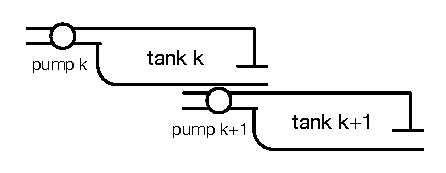
\includegraphics[clip=true,trim=0.3cm 0.35cm 0.3cm 0.35cm,width=0.7\columnwidth]{water.pdf}    
\caption{Connected water tanks.}  \label{fig:water}
\end{figure}

The safety property is that the water level of each tank is in a certain range
$I = [L_m - \eta, L_M + \eta]$.
%
We have verified this safety property for  \emph{any number} of connected water tanks 
using inductive and compositional analysis.%
\footnote{For a tank $k$ and %a subinterval 
$I' = [L_m - \eta', L_M + \eta']\subseteq I$ with $\eta' < \eta$,
provided  that $x_{k-1} \in I$ always holds, % for its input tank  $k-1$.
we show that $x_{k} \in I'$ is an inductive condition,
and  $x_{k} \in I$ always holds
if $x_{k} \in I'$ at the beginning of each round
(i.e., $(x_k(0) \in I' \wedge \phi_{\mathcal{E} \restriction_{\Pi}
  E_\mathcal{E}}^{T,0}) \rightarrow (x_k(T) \in I') \wedge (\forall t
\in [0,T].\; x_{k}(t) \in I)$).} 
%
For  maximal clock skew $\epsilon = 30\,\mathrm{ms}$,
 sampling time $t_I = 20\,\mathrm{ms}$,
and  response time $t_R = 100\,\mathrm{ms}$,
we have proved the  compositional safety property
% for any number of water tanks
% by checking the unsatisfiability of the negated formulas,
 using \textsf{dReal} with precision $\delta = 0.001$ (the analysis took $4.3$ seconds).%
 \footnote{In the analysis, we use the parameters 
$a = 0.5$, $b = 0.6$, $g = 9.8$, $A = 2$, $q = 4$, $L_m = 8$, $L_M = 10$,
$\eta = 3$, $\eta' = 2$, and $T = 1\,\mathrm{s}$.}
However, if $\epsilon = 150\,\mathrm{ms}$,
then the compositional inductive condition is violated by the trajectory in Fig.~\ref{fig:water-error}
%generated by \textsf{dReal} with precision $\delta = 0.001$
(the analysis took $1.46$ seconds).

\begin{figure}
\centering
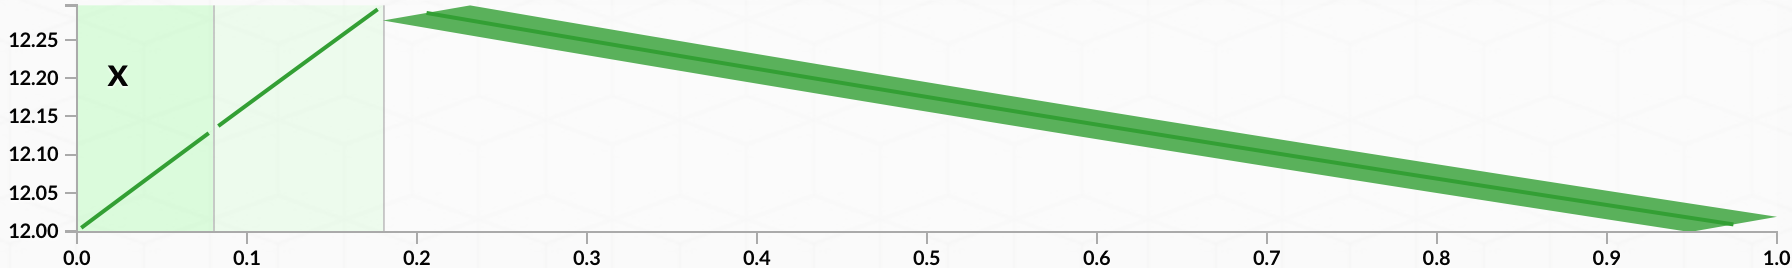
\includegraphics[clip=true,trim=1ex 1ex 1ex 1ex,width=\columnwidth]{water-error.png}    
\caption{The counterexample trajectory when $\epsilon = 150\,\mathrm{ms}$,
where the water level increases for extra $300\,\mathrm{ms}$ to violate the inductive condition. % at the end of the round.
} \label{fig:water-error}
\end{figure}





\subsection{Networked Thermostat Controllers}

%A classical thermostat controller  \cite{henzinger2000theory} is installed in each room.
%(where the specification of a single hybrid automaton is adapted from \cite{henzinger2000theory}). 
A number of rooms are interconnected by open doors, 
as shown in Fig.~\ref{fig:adj-rooms}.
The temperature of each room is separately controlled by its own
thermostat controller that turns the heater on and off.
That is, it %The temperature of each room 
depends on
the heater's mode $m \in \{m_\texttt{on}, m_\texttt{off}\}$  and the temperatures of the other rooms.
The temperature $x_i$ of room $i$
changes according to the ODEs:%
\footnote{%where 
$K_i, h_i \in \mathbb{R}$ are constants depending on
the size of room $i$ and the heater's power, respectively,
and $c \in \mathbb{R}$ is determined by the size of the open door.}
\begin{align*}
\dot{x}_i &= K_i (h_i - ((1- 2 c) x_i + c x_{i-1} + c x_{i+1})) &&\mbox{if}\; m_i = m_\texttt{on}
\\
\dot{x}_i &= - K_i ((1- 2 c) x_i + c x_{i-1} + c x_{i+1}) && \mbox{if}\; m_i = m_\texttt{off}
\end{align*}
%
In each transition, a controller turns on the heater 
 if $x_i \leq T_m$,
and turns it  off if $x_i > T_M$.

\begin{figure}
\centering
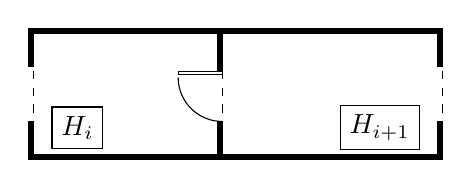
\begin{tikzpicture}[scale=0.8] %baseline=(current bounding box.north)
%left wall
\filldraw  (-3,0.08) rectangle  + (-0.08,-0.6)
	(-3,-2.0) rectangle  + (-0.08,0.6);
\draw[dashed] (-3,-0.6) -- (-3,-2);
%room1
\filldraw (0,0) rectangle  + (-3,0.08)
	(-3.08,-2.0) rectangle  + (3,0.08);
\path (-2.3,-1.5) node[draw] { $H_i$};
%wall
\filldraw (0,-0.6) rectangle  + (-0.08,0.6)
	(0,-2.0) rectangle  + (-0.08,0.6);
\draw[dashed] (0,-0.6) -- (0,-2);
%door
\draw (0,-0.6) rectangle +(-0.7,-0.05);
\draw (-0.7,-0.7) arc (180:270:0.7);
%room2
\filldraw (0,0) rectangle  + (3.5,0.08)
	(3.5,-2.0) rectangle  + (-3.5,0.08);
\path (2.5,-1.5) node[draw] (m2){ $H_{i+1}$};
%right wall
\filldraw  (3.5,0.08) rectangle  + (-0.08,-0.6)
	(3.5,-2.0) rectangle  + (-0.08,0.6);
\draw[dashed] (3.5,-0.6) -- (3.5,-2);
\end{tikzpicture}
\caption{Interconnected rooms. %  by an open door.
} \label{fig:adj-rooms}
\end{figure}

The safety property is that the temperature of each room
is in the range $I = [T_m - \eta, T_M + \eta]$.
We have verified the safety property $\forall t.\; x_i \in I$
for  \emph{any number} of interconnected thermostat controllers
by inductive and compositional analysis.%
\footnote{For %a subinterval 
$I' = [T_m - \eta', T_M + \eta']\subseteq I$,
provided that both $x_{i-1} \in I$ and $x_{i+1} \in I$ always hold,
we show that $x_i \in I'$ is an inductive condition,
and $x_i \in I$ always holds
if $x_i \in I'$ at the beginning of each round.}
%
For $\epsilon = 2\,\mathrm{ms}$,
$t_I = 10\,\mathrm{ms}$,
and $t_R = 200\,\mathrm{ms}$,
we have proved (in $2.6$ seconds) the compositional safety property 
%for any number of thermostats 
%by checking the unsatisfiability of the negated formulas,
 using \textsf{dReal} with precision $\delta = 0.001$.\footnote{In the analysis, we use the parameters $K = 0.015$, 
$h = 100$,
$c = 0.01$,
$T_M = 21$, 
$T_m = 19$,
$\eta = 3$, $\eta' = 2$,
and $T = 1\,\mathrm{s}$.}
%
However, if $\epsilon = 20\,\mathrm{ms}$,
then the compositional inductive condition is violated by the trajectory in Fig.~\ref{fig:thermo-error}
(the analysis took $0.56$ seconds).


\begin{figure}
\centering
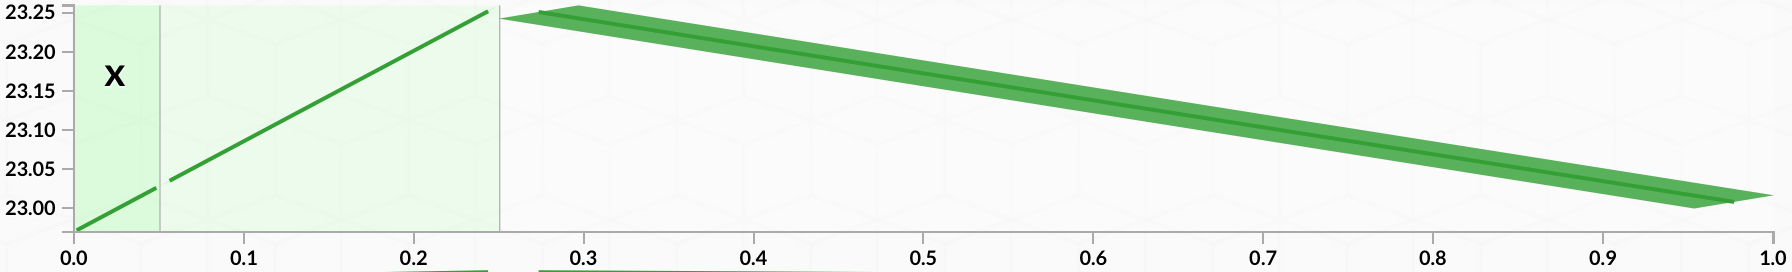
\includegraphics[clip=true,trim=1ex 1ex 1ex 1ex,width=\columnwidth]{thermo-error.png}    
\caption{The counterexample trajectory when $\epsilon = 20\,\mathrm{ms}$.
%where the temperature  rises for extra $20\,\mathrm{ms}$ and thus $x > 23$ at the end of the round.
} \label{fig:thermo-error}
\end{figure}


%\subsection{Automated Highway System}
%
%...

%\subsection{Quadrotor Attitude Controller}
%\label{sec:quadrotor}
%..

%\subsection{Steam Boiler Controller}
%...

\subsection{Bounded Reachability Comparison}
\label{sec:expr}

We have implemented the SMT algorithm
for our new logic $\mathcal{L}_{\mathcal{F}\cup\mathcal{N}}$ in the \textsf{dReal} SMT solver \cite{dReal},
and have compared the performance of 
the new $\mathcal{L}_{\mathcal{F}\cup\mathcal{N}}$-encoding
with one of the previous \emph{non-modular} $\mathcal{L}_{\mathcal{F}}$-encoding  for Hybrid PALS models.
%
In this comparison,
we only consider special cases %of the examples 
with no clock skews ($\epsilon = 0$) 
due to a lack of expressiveness of  $\mathcal{L}_{\mathcal{F}}$,
and only bounded reachability analysis
since it needs to generate bigger formulas than other types of analysis.


We have performed bounded reachability analysis up to $k = 5$
for the safety properties for the ``concrete'' instances of the case studies
(using \textsf{dReal} without the use of other SMT heuristics).
The results for $k$-step bounded reachability analysis 
are summarized  in Fig.~\ref{table:bounded} and show that
%
the new encoding significantly outperforms 
the non-modular encoding.\footnote{We consider both \texttt{unsat} (verified) and \texttt{sat}  (counterexample found) cases
by using different safety properties.}
For example, 
the SMT analysis using the non-modular encoding
for  three interconnected thermostats
 did not terminate for $30$ hours
even for $k = 2$.


\begin{figure}
\centering
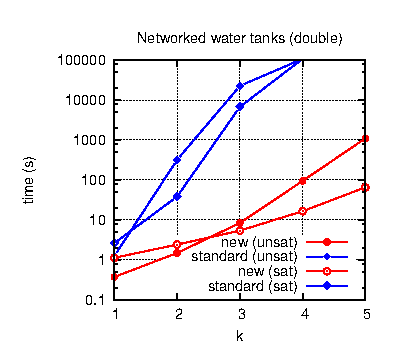
\includegraphics[width=0.45\columnwidth]{plot/water-double.eps}    
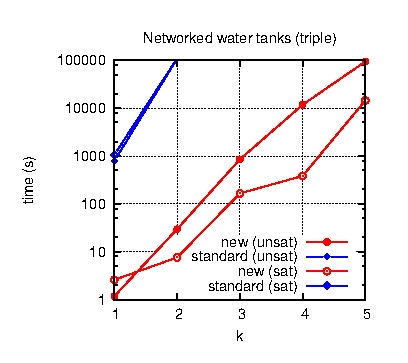
\includegraphics[width=0.45\columnwidth]{plot/water-triple.eps}    
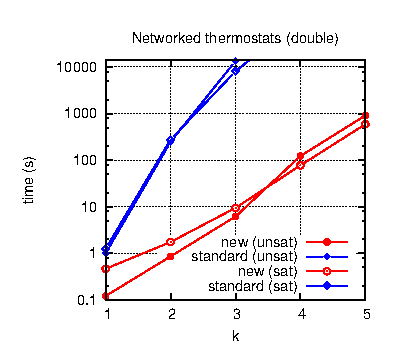
\includegraphics[width=0.45\columnwidth]{plot/thermostat-double.eps}    
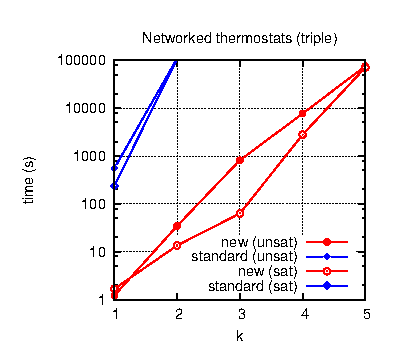
\includegraphics[width=0.45\columnwidth]{plot/thermostat-triple.eps}    
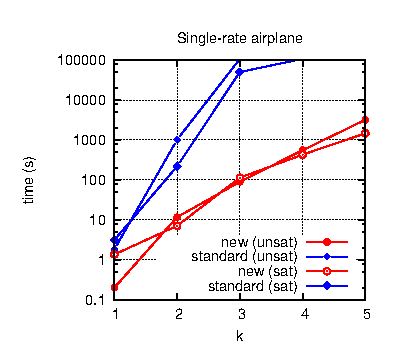
\includegraphics[width=0.45\columnwidth]{plot/airplane-single.eps}    
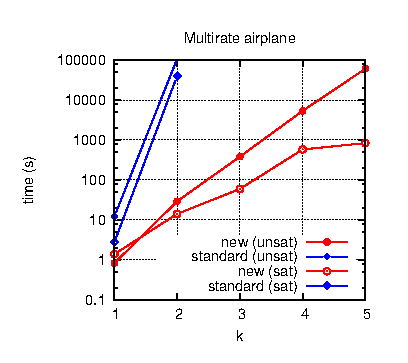
\includegraphics[width=0.45\columnwidth]{plot/airplane-multi.eps}    
\caption{Running time of $k$-step bounded reachability analysis, where red lines denote the new encoding,
and blue lines denote the non-modular encoding.}
\label{table:bounded}
\end{figure}






% !TEX root = /Users/kquine/Dropbox/Research/Papers/2015/CPS-SMT-RTSS/cps-rtss.tex


\section{Related Work}
\label{sec:related-work}

%many important advances have been made by
%various approaches, including \cite{DBLP:journals/jlp/FranzleTE10,DBLP:conf/cav/FrehseGDCRLRGDM11,DBLP:journals/tac/AlthoffK14,frehse2005phaver,DBLP:conf/icons/HerdeEFT08,DBLP:conf/rtss/ChenAS12,DBLP:conf/aaai/CimattiMT12,platzer2008differential}.

%PALS was originally proposed to reduce the system complexity of 
%single-rate virtually synchronous distributed real-time systems \cite{pals-rtss09,pals-tcs},
%and then extended for multirate systems \cite{mr-pals-journal,al2012pattern} and hybrid systems \cite{ftscs-journal,hybrid-pals}.

%%% Peter: I have no clue what the following section was doing in the
%%% paper ...
% Hybrid automata techniques are not appropriate for hybrid PALS models.
% Hybrid PALS models are basically time triggered models, which are not perfectly synchronized due to clock skews,
% whereas composing hybrid automata requires perfect synchronization of several events.

%%% (Peter): I try to add some PALS rel work. 
PALS~\cite{pals-rtss09,mr-pals-journal,pals-tcs,al2012pattern} targets
distributed real-time systems, whose absence of continuous behaviors
means that continuous behaviors and local clocks do not need to be
taken into account in the synchronous models, which can therefore be
verified by any explicit-state model checker. In contrast, Hybrid PALS
synchronous models must take both clock skews and continuous behaviors
into account and hence cannot be analyzed by explicit-state
techniques. The first steps to add continuous behaviors to PALS were
taken in~\cite{hybrid-pals}. The present work presents a more general
model, where the relative sampling and actuating times are system
parameters,  and also provides a crucial bisimulation result between
the 
synchronous and the distributed model. But the main difference is in the
verification part. \textbf{Kyungmin, add stuff here!!!}


Because of the difficulty of handling SMT
formulas over the reals with nonlinear functions, 
SMT-solving-based verification is a fairly new direction for nonlinear hybrid
systems. The research
direction is initiated in~\cite{ratschan2007safety}, which uses constraint
solving algorithms for handling nonlinear reachability problems. Two
main lines of work that explicitly formulate problems as SMT formulas
are based on the HySAT/iSAT
solver~\cite{DBLP:journals/fmsd/FranzleH07,eggers2008sat}
and the MathSAT
solver~\cite{DBLP:conf/aaai/CimattiMT12,DBLP:conf/fmcad/CimattiMT12}.
But efficient encoding of networks of hybrid systems has not been
investigated in existing work along these lines. 

On the other hand,
for reachable set computation, 
%the work on 
SpaceEX~\cite{DBLP:conf/cav/FrehseGDCRLRGDM11}
has involved methods for handling networks restricted to linear/multiaffine hybrid systems,
and 
Flow*~\cite{DBLP:conf/cav/ChenAS13} proposed an approach for verifying
nonlinear hybrid systems using Taylor model flowpipe construction. 
%
dReach~\cite{dReach}
encodes reachability problems of hybrid systems to SMT problems and
solves them using %a $\delta$-decision procedures, 
dReal~\cite{dReal}.
%
Our approach is different from dReach, 
since dReach \emph{explicitly} enumerates all mode paths of a hybrid automaton
to generate many small SMT formulas for these paths.



%Multirate PALS ?? ( Abdullah's work, other synchronizer, virtually synchronization, ...)
%SMT and \texttt{dReal} ??



% !TEX root = /Users/kquine/Dropbox/Research/Papers/2015/CPS-SMT-RTSS/cps-rtss.tex

\section{Concluding Remarks}
\label{sec:concl}

..


\bibliographystyle{IEEEtran}
\bibliography{kbae-bib}

%\appendix
%% !TEX root = /Users/kquine/Dropbox/Research/Papers/2015/CPS-SMT-RTSS/cps-rtss.tex


\section{PALS Definitions}
\label{sec:pals-defs}




\begin{definition}
 For a typed machine $M_j = (D_{i_j}, S_j, D_{o_j}, \delta_{M_j})$ with 
 input set $D_{i_j} = D_{i_{j_1}} \times \cdots \times D_{i_{j_n}}$, an input adaptor
 $\mathit{adap}(j)=\{\alpha_i: D'_l \rightarrow D_{i_l}\}_{l\in\{1,\ldots, n_j\}}$
 is a family of functions to give desired input values
 $(\alpha_1(d_1),\ldots,\alpha_n(d_n))$ %for $M_j$'s input ports 
 from output $(d_1,\ldots,d_n) \in D_1 \times \cdots \times D_n$ of other machines.  
\end{definition}


\begin{definition}
A \emph{multirate machine ensemble} is 
given by
a tuple
$\mathcal{E} = (J_S ,  J_F, e, \{M_j\}_{j\in J_S \cup J_F}, E, \mathit{src}, \mathit{rate}, \mathit{adap})$
with:
\begin{inparaenum}[(i)]
	\item $J_S$ a set of slow machine indices;
	\item $J_F$ a set of fast machine indices ($J_S \cap J_F = \emptyset$);
	\item $e\not\in J_S \cup J_F$ the environment index;
 	\item $\{M_j\}_{j\in J_S \cup J_F}$  a family of typed machines;
	\item $E=(D^e_i, D^e_o)$ 
	the \emph{environment} with $D^{e}_i$  the \emph{input set} and 
	$D^{e}_o$  the \emph{output set};
	\item $\mathit{src}$  a \emph{wiring diagram} assigning to each input port its source output port, 
	 so that no connection exists between two ``fast'' machines;
	\item $\mathit{rate}$ assigning to a fast 
	machine its \emph{rate};
	%denoting how many times faster than the slow machines it is; 
	and
	\item $\mathit{adap}$ assigning to a machine its \emph{input adaptor}.
	%for  communication between components with different rates.
\end{inparaenum}
\end{definition}

\begin{definition}
The \emph{synchronous composition}
of  an ensemble
$\mathcal{E} = (J_S, J_F, e, \{M_j\}_{j\in J_s \cup J_F}, E, \mathit{src}, \mathit{rate}, \mathit{adap})$
is the typed machine
$ M_{\mathcal{E}} = ( D_i^{\mathcal{E}}, S^{\mathcal{E}},D_o^{\mathcal{E}}, \delta_{\mathcal{E}})$
where:
\begin{inparaenum}[(i)]
	\item $D_i^{\mathcal{E}} = D^e_o$ and  $D_o^{\mathcal{E}} = D^e_i$;
	\item $S^{\mathcal{E}} = (\Pi_{j\in J} S_j) \times (\Pi_{j\in J} D_{OF}^j)$, 
	where
	$D^j_{OF}$ stores the ``feedback outputs'' of subcomponents; and
	\item $ \delta_{\mathcal{E}} \subseteq 
	(D^{\mathcal{E}}_i\times S^{\mathcal{E}}) \:\times \: (S^{\mathcal{E}} \times D_o^{\mathcal{E}})$
	``combines''  the  transitions of the subcomponents
	 into a synchronous step (see \cite{pals-tcs}).
\end{inparaenum}
\end{definition}

\begin{definition}
The transition system for an ensemble $\mathcal{E}$ is a pair 
$\mathit{ts}(\mathcal{E}) = (S^{\mathcal{E}} \times \mathcal{D}_i^{\mathcal{E}}, \longrightarrow_{\mathcal{E}})$,
where $(\vec{s}_1,\vec{i}_1) \longrightarrow_{\mathcal{E}} (\vec{s}_2,\vec{i}_2)$
iff an ensemble in state $\vec{s}$ and with input
$\vec{i}$ from the environment has a transition to state $\vec{s'}$
(i.e., $\exists \vec{o}.\; ((\vec{i}, \vec{s}), (\vec{s'}, \vec{o})) \in \delta_{\mathcal{E}}$)
and the environment can generate output $\vec{i'}$ in the next step.
\end{definition}


\begin{definition}  
Consider $n$ controlled physical environments
$E_{M_i} = (C_i, {\vec{x}}_i, \Lambda_i)$
with $\vec{x}_i =  (x_{i_1}, \ldots,x_{i_{l_i}})$
for $i = 1,\ldots,n$.
Given a variable $t$ for time,
a \emph{time-invariant constraint}
is a logic formula of the form  
$(\forall t)\; \psi(\vec{x}_1(t), \vec{x}_2(t), \ldots, \vec{x}_n(t))$.
\end{definition}


\end{document}
